\chapter{Maxwell 近场与球形散射}
\label{chap:maxwell-general}
\label{chap:maxwell-applications}

电子方程已经说明给定外场怎样产生相位，但并不能告诉我们纳米结构表面究竟有什么电场。要从材料参数和照明条件真正计算耦合，就必须先解产生近场的 Maxwell 边值问题。Green 张量给出任意源的辐射场；散射算符则将材料响应与自由空间传播分开。对材料和几何的处理在此完成，电子侧仍沿用已经建立的轨迹投影，不再重复推导边带。

把材料参数转化成可测的边带，需要完成以下连续计算：
\begin{equation}
{
\text{材料与几何}
\longrightarrow
\vb E_\omega
\longrightarrow
\beta[\vb E_\omega]
\longrightarrow
J_n^2(2|\beta|).}
\label{eq:maxwell-to-pinem-chain}
\end{equation}
Green 张量、\(T\) 算符、VSH、Mie 系数和 Rayleigh 极限都只服务于第一支箭头；电子响应从头到尾不变。

在均匀宿主中，波矢满足 $k_\parallel^2+k_\perp^2=(n_\mathrm h\omega/c)^2$。当 $v_0<c/n_\mathrm h$，相位匹配 $k_\parallel=\omega/v_0$ 要求横向倏逝波数
\begin{equation}
\chi_\perp=\sqrt{(\omega/v_0)^2-(n_\mathrm h\omega/c)^2},
\label{eq:evanescent-decay-from-kinematics}
\end{equation}
这说明局域近场与自由传播光为何具有不同的电子耦合效率。这里 $n_\mathrm h$ 表示无耗散宿主的折射率；有耗散时应在复波数及其满足辐射条件的分支上继续推导。


这里直接从矢量 Maxwell 方程建立母算符；标量 Helmholtz Green 函数只作为同一逆算符思想的数学预备，不参与电磁母理论的建立，其 Fourier/留数推导可由一般几何模型另行处理。


\section{Maxwell 散射算符}
先不假定任何几何对称性。把 Maxwell 方程抽象地写成
\begin{equation}
\mathcal L\vb E=\vb S,
\end{equation}
并找到满足
\begin{equation}
\mathcal L\mathbf G(\vb r,\vb r')=\mathbf I\delta(\vb r-\vb r')
\end{equation}
的核，那么把第二式乘以 $\vb S(\vb r')$ 并对 $\vb r'$ 积分，就有
\begin{align}
\mathcal L\int\mathbf G(\vb r,\vb r')\cdot\vb S(\vb r')\dd^3r'
&=\int\mathbf I\delta(\vb r-\vb r')\cdot\vb S(\vb r')\dd^3r'\\
&=\vb S(\vb r).
\end{align}
因此
\begin{equation}
\vb E(\vb r)=\int\mathbf G(\vb r,\vb r')\cdot\vb S(\vb r')\dd^3r'
\end{equation}
只是 $\vb E=\mathcal L^{-1}\vb S$ 的坐标表示。下面所做的 dyadic Green 理论只是把这个初等事实应用到矢量 Maxwell 算符。

对任意形状，把“Maxwell 求场”和“电子沿轨迹取相位匹配分量”写成两个线性算符。母问题允许局域、线性、各向异性的相对介电张量与相对磁导率张量
\begin{equation}
 \boldsymbol\varepsilon(\vb r,\omega),
 \qquad
 \boldsymbol\mu(\vb r,\omega),
\end{equation}
它们都可以是复数和频散的。非局域介质需要把下面的乘法本构张量进一步提升为积分核，但电子探测泛函本身不变。采用 $\ee^{-\ii\omega t}$ 约定，并记
\begin{equation}
k_{\rm vac}\equiv\frac{\omega}{c},
\end{equation}
以避免与电子中心波数 $k_0$ 冲突。频域 Maxwell 方程为
\begin{align}
\nabla\times\vb E
&=\ii\omega\mu_0\boldsymbol\mu\cdot\vb H,
\label{eq:maxwell-curl-E-general}\\
\nabla\times\vb H
&=\vb J_{\rm ext}
-\ii\omega\varepsilon_0\boldsymbol\varepsilon\cdot\vb E.
\label{eq:maxwell-curl-H-general}
\end{align}
由第一式
\begin{equation}
 \vb H
 =\frac{1}{\ii\omega\mu_0}
 \boldsymbol\mu^{-1}\cdot(\vb\nabla\times\vb E).
\end{equation}
代入第二式：
\begin{align}
\frac{1}{\ii\omega\mu_0}
\vb\nabla\times
\boldsymbol\mu^{-1}\cdot(\vb\nabla\times\vb E)
&=\vb J_{\rm ext}
-\ii\omega\varepsilon_0\boldsymbol\varepsilon\cdot\vb E.
\end{align}
两边乘以 $\ii\omega\mu_0$，并利用 $c^{-2}=\mu_0\varepsilon_0$：
\begin{equation}
 {
 \left[
 \vb\nabla\times\boldsymbol\mu^{-1}(\vb r,\omega)\cdot\vb\nabla\times
 -k_{\rm vac}^2\boldsymbol\varepsilon(\vb r,\omega)
 \right]\vb E
 =\ii\omega\mu_0\vb J_{\rm ext}.}
 \label{eq:Maxwell_general}
\end{equation}
这里两个旋度之间的 $\boldsymbol\mu^{-1}$ 是位置依赖算符乘法，不能在一般非均匀磁介质中移到旋度外。定义 Maxwell 算符
\begin{equation}
 \mathcal L
 \equiv
 \vb\nabla\times\boldsymbol\mu^{-1}\cdot\vb\nabla\times
 -k_{\rm vac}^2\boldsymbol\varepsilon,
 \label{eq:general-maxwell-operator}
\end{equation}
以及满足相同外向辐射条件的 dyadic Green 张量
\begin{equation}
{
\mathcal L\,\mathbf G(\vb r,\vb r';\omega)
=\mathbf I\,\delta(\vb r-\vb r').}
\label{eq:dyadicGreenDef}
\end{equation}
当 $\boldsymbol\mu=\mathbf I$ 时立即退化为通常的
$\vb\nabla\times\vb\nabla\times-k_{\rm vac}^2\boldsymbol\varepsilon$ 形式。
则显式外源产生的场为
\begin{equation}
{
\vb E(\vb r,\omega)
=\ii\omega\mu_0
\int\dd^3r'\,\mathbf G(\vb r,\vb r';\omega)\cdot\vb J_{\rm ext}(\vb r',\omega).}
\label{eq:E_GJ}
\end{equation}


一般介质的 Maxwell 算符已经定义。均匀宿主提供一个可以完全算出的逆算符：在 Fourier 空间，纵向场与横向场分别受到不同的投影作用，这使 Green 张量的辐射边界条件也能够被明确追踪。


对均匀、各向同性宿主，$\boldsymbol\varepsilon=\varepsilon_{\rm h}\mathbf I$、$\boldsymbol\mu=\mu_{\rm h}\mathbf I$，其中 $\varepsilon_{\rm h},\mu_{\rm h}$ 可以是复数，但在空间中为常数。定义
\begin{equation}
 k_{\rm h}^2=k_{\rm vac}^2\varepsilon_{\rm h}\mu_{\rm h},
 \qquad
 \mathbf P_{\rm L}(\vb k)=\hat{\vb k}\hat{\vb k},
 \qquad
 \mathbf P_{\rm T}(\vb k)=\mathbf I-\mathbf P_{\rm L}(\vb k).
 \label{eq:LT-projectors}
\end{equation}
在 Fourier 空间中 $\vb\nabla\to\ii\vb k$，因而
\begin{align}
\vb\nabla\times\vb\nabla\times\vb E
&\longrightarrow
-\vb k\times(\vb k\times\widetilde{\vb E})\\
&=\left(k^2\mathbf I-\vb k\vb k\right)\cdot\widetilde{\vb E}\\
&=k^2\mathbf P_{\rm T}\cdot\widetilde{\vb E}.
\end{align}
把 $\mathbf I=\mathbf P_{\rm T}+\mathbf P_{\rm L}$ 代入
$\mathcal L_{\rm h}=\mu_{\rm h}^{-1}\vb\nabla\times\vb\nabla\times-k_{\rm vac}^2\varepsilon_{\rm h}$，得到
\begin{align}
\widetilde{\mathcal L}_{\rm h}
&=\left(\frac{k^2}{\mu_{\rm h}}-k_{\rm vac}^2\varepsilon_{\rm h}\right)\mathbf P_{\rm T}
-k_{\rm vac}^2\varepsilon_{\rm h}\mathbf P_{\rm L}\\
&=\frac{k^2-k_{\rm h}^2}{\mu_{\rm h}}\mathbf P_{\rm T}
-\frac{k_{\rm h}^2}{\mu_{\rm h}}\mathbf P_{\rm L}.
\label{eq:maxwell-LT-decomposition}
\end{align}
由于 $\mathbf P_{\rm T}\mathbf P_{\rm L}=0$ 且 $\mathbf P_{\rm T,L}^2=\mathbf P_{\rm T,L}$，令
$\widetilde{\mathbf G}_{\rm h}=A\mathbf P_{\rm T}+B\mathbf P_{\rm L}$，则
\begin{equation}
\widetilde{\mathcal L}_{\rm h}\widetilde{\mathbf G}_{\rm h}
=\frac{k^2-k_{\rm h}^2}{\mu_{\rm h}}A\mathbf P_{\rm T}
-\frac{k_{\rm h}^2}{\mu_{\rm h}}B\mathbf P_{\rm L}.
\end{equation}
要求它等于 $\mathbf I=\mathbf P_{\rm T}+\mathbf P_{\rm L}$，逐个投影通道比较系数：
\begin{equation}
 A=\frac{\mu_{\rm h}}{k^2-k_{\rm h}^2-\ii0^+},
 \qquad
 B=-\frac{\mu_{\rm h}}{k_{\rm h}^2}.
\end{equation}
所以
\begin{equation}
 {
 \widetilde{\mathbf G}_{\rm h}(\vb k;\omega)
 =\mu_{\rm h}\left[
 \frac{\mathbf P_{\rm T}(\vb k)}{k^2-k_{\rm h}^2-\ii0^+}
 -\frac{\mathbf P_{\rm L}(\vb k)}{k_{\rm h}^2}
 \right].}
 \label{eq:homogeneous-green-k}
\end{equation}
其中 $-\ii0^+$ 与 $\ee^{-\ii\omega t}$ 约定对应外向辐射边界条件。第一项包含传播的横向 Maxwell 极点，第二项是纵向约束部分；后者没有光锥极点。非磁宿主只需令 $\mu_{\rm h}=1$，而不是重新建立另一套公式。

实空间形式从标量 Helmholtz Green 函数
\begin{equation}
 g_{\rm h}(R)=\frac{\ee^{\ii k_{\rm h}R}}{4\pi R},
 \qquad
 (\nabla^2+k_{\rm h}^2)g_{\rm h}=-\delta(\vb R),
 \qquad
 \vb R=\vb r-\vb r',
 \label{eq:scalar-helmholtz-green}
\end{equation}
构造为
\begin{equation}
 {
 \mathbf G_{\rm h}(\vb R)
 =\mu_{\rm h}\left(\mathbf I+\frac{\vb\nabla\vb\nabla}{k_{\rm h}^2}\right)
 g_{\rm h}(R).}
 \label{eq:dyadic-from-scalar}
\end{equation}
对 $R\neq0$，径向函数满足
\begin{equation}
 \partial_i\partial_j g
 =\left(g''-\frac{g'}{R}\right)\hat R_i\hat R_j
 +\frac{g'}{R}\delta_{ij}.
\end{equation}
由
\begin{align}
 g'&=g\left(\ii k_{\rm h}-\frac1R\right),\\
 g''&=g\left(-k_{\rm h}^2-\frac{2\ii k_{\rm h}}R+\frac{2}{R^2}\right),
\end{align}
代回式~\cref{eq:dyadic-from-scalar}，得到显式 dyadic Green 张量
\begin{equation}
 {
 \mathbf G_{\rm h}(\vb R)
 =\mu_{\rm h}\frac{\ee^{\ii k_{\rm h}R}}{4\pi R}
 \left\{
 \left[1+\frac{\ii k_{\rm h}R-1}{k_{\rm h}^2R^2}\right]\mathbf I
 +\left[-1-\frac{3\ii}{k_{\rm h}R}
 +\frac{3}{k_{\rm h}^2R^2}\right]
 \hat{\vb R}\hat{\vb R}
 \right\}.}
 \label{eq:homogeneous-green-real}
\end{equation}
所以同一个 Green 张量自动包含三个空间尺度：
\begin{equation}
 \mathbf G_{\rm h}
 \sim
 \begin{cases}
 R^{-3},&|k_{\rm h}|R\ll1\quad\text{准静态近场},\\
 R^{-2},&|k_{\rm h}|R\sim1\quad\text{感应区},\\
 R^{-1},&|k_{\rm h}|R\gg1\quad\text{辐射远场}.
 \end{cases}
 \label{eq:green-three-zones}
\end{equation}
式~\cref{eq:homogeneous-green-real} 的 $R^{-3}$ 部分给出准静态偶极近场，而球形 Mie 展开在球对称条件下保留全部 $\ell$ 与全部 $k_{\rm h}R$ 阶数。

在非磁介质特例中，介电散射势也可以从“感生极化电流”角度重新得到。定义
\begin{equation}
 \vb P_{\rm ind}
 =\varepsilon_0\Delta\boldsymbol\varepsilon\cdot\vb E,
 \qquad
 \vb J_{\rm ind}
 =\partial_t\vb P_{\rm ind}
 \longrightarrow-\ii\omega\vb P_{\rm ind}.
 \label{eq:induced-current}
\end{equation}
代入式~\cref{eq:E_GJ}：
\begin{align}
\vb E_{\rm sc}
&=\ii\omega\mu_0\mathbf G_{\rm h}\vb J_{\rm ind}\\
&=\omega^2\mu_0\varepsilon_0
\mathbf G_{\rm h}\Delta\boldsymbol\varepsilon\vb E\\
&=k_{\rm vac}^2
\mathbf G_{\rm h}\Delta\boldsymbol\varepsilon\vb E,
\end{align}
这与下面 $\mathbf G_{\rm h}\mathbf V\vb E$ 完全一致。因此 $\mathbf V=k_{\rm vac}^2\Delta\boldsymbol\varepsilon$ 不是形式定义，而是 Maxwell 极化电流重新辐射的紧凑写法。

若介质满足局域互易条件
\begin{equation}
 \boldsymbol\varepsilon^{\mathsf T}(\vb r,\omega)
 =\boldsymbol\varepsilon(\vb r,\omega),
 \qquad
 \boldsymbol\mu^{\mathsf T}(\vb r,\omega)
 =\boldsymbol\mu(\vb r,\omega),
 \label{eq:reciprocal-epsilon}
\end{equation}
则 Maxwell 算符在不含复共轭的双线性 Green 恒等式下是对称的。取两个点源解 $\mathbf G(\cdot,\vb r_1)\cdot\vb a$ 与
$\mathbf G(\cdot,\vb r_2)\cdot\vb b$，对包围所有散射体的体积应用旋度 Green 恒等式，外向边界项成对抵消，得到
\begin{equation}
 \vb a\cdot\mathbf G(\vb r_1,\vb r_2)\cdot\vb b
 =\vb b\cdot\mathbf G(\vb r_2,\vb r_1)\cdot\vb a.
\end{equation}
由于 $\vb a,\vb b$ 任意，
\begin{equation}
 {
 \mathbf G(\vb r,\vb r';\omega)
 =\mathbf G^{\mathsf T}(\vb r',\vb r;\omega).}
 \label{eq:green-reciprocity}
\end{equation}
这使“光场激发结构再由电子探测”和“把电子轨迹视作测试源再反向投影到光学激发”成为同一个互易散射核的两种读法。

为了把电子模块写成与坐标选择无关的形式，定义电子探测线性泛函
\begin{equation}
{
\mathcal L_{\rm e}[\vb E]
\equiv
\int_{-\infty}^{+\infty}\dd s\,
\hat{\vb v}_0\cdot
\vb E(\vb R_\perp+s\hat{\vb v}_0,\omega)
\ee^{-\ii\kappa s},
\qquad
\kappa\equiv\frac{\omega}{v_0}.}
\label{eq:electron-detection-functional}
\end{equation}
于是式~\cref{eq:Fparallel-general-def} 简写为
\begin{equation}
{
\mathcal F_{\parallel}^{\rm tot}=\mathcal L_{\rm e}[\vb E_{\rm inc}+\vb E_{\rm sc}]
=\mathcal F_{\parallel}^{\rm inc}+\mathcal F_{\parallel}^{\rm sc}.}
\label{eq:F-as-functional}
\end{equation}
电子端只认识最终的 $\mathcal F_{\parallel}^{\rm tot}$；具体 Maxwell 求解器的任务只是计算其中的场。若入射场轨迹投影为零，则可把 $\mathcal F_{\parallel}^{\rm sc}$ 简写为 $\mathcal F_{\parallel}$。


若从入射场出发，选均匀各向同性宿主 $(\varepsilon_{\rm h},\mu_{\rm h})$，其 Green 张量记为 $\mathbf G_{\rm h}$。先定义
\begin{equation}
 \Delta\boldsymbol\varepsilon
 \equiv\boldsymbol\varepsilon-\varepsilon_{\rm h}\mathbf I,
 \qquad
 \Delta\boldsymbol\mu^{-1}
 \equiv\mu_{\rm h}^{-1}\mathbf I-\boldsymbol\mu^{-1}.
\end{equation}
宿主算符为
\begin{equation}
 \mathcal L_{\rm h}
 =\vb\nabla\times\mu_{\rm h}^{-1}\vb\nabla\times
 -k_{\rm vac}^2\varepsilon_{\rm h}\mathbf I.
\end{equation}
为了保持 $\mathcal L=\mathcal L_{\rm h}-\mathbf V$，一般电磁散射势必须写成算符
\begin{equation}
 {
 \mathbf V
 =\vb\nabla\times\Delta\boldsymbol\mu^{-1}\cdot\vb\nabla\times
 +k_{\rm vac}^2\Delta\boldsymbol\varepsilon.}
 \label{eq:general-electromagnetic-scattering-potential}
\end{equation}
第一项描述磁导率对比，第二项描述介电对比。只有在粒子和宿主都非磁、$\boldsymbol\mu=\mu_{\rm h}\mathbf I=\mathbf I$ 时，第一项才严格消失，并退化为常用的局域乘法算符
\begin{equation}
 {\mathbf V=k_{\rm vac}^2\Delta\boldsymbol\varepsilon.}
 \label{eq:dielectric-scattering-potential}
\end{equation}
在没有显式体源、只有给定入射场时，$\mathcal L\vb E=0$，故
\begin{align}
(\mathcal L_{\rm h}-\mathbf V)\vb E&=0,\\
\mathcal L_{\rm h}\vb E&=\mathbf V\vb E.
\end{align}
另一方面 $\mathcal L_{\rm h}\vb E_{\rm inc}=0$。因此 $\vb E-\vb E_{\rm inc}$ 满足
\begin{equation}
\mathcal L_{\rm h}(\vb E-\vb E_{\rm inc})=\mathbf V\vb E.
\end{equation}
左乘宿主 Green 算符 $\mathbf G_{\rm h}=\mathcal L_{\rm h}^{-1}$，并选取相同的外向辐射边界条件，得到 Lippmann--Schwinger 方程
\begin{equation}
{
\vb E=\vb E_{\rm inc}+\mathbf G_{\rm h}\mathbf V\vb E.}
\label{eq:LS-operator}
\end{equation}
在非磁介电对比特例~\cref{eq:dielectric-scattering-potential} 下，坐标形式才简化为
\begin{equation}
\vb E(\vb r)=\vb E_{\rm inc}(\vb r)
+k_{\rm vac}^2\int_V\dd^3r'\,
\mathbf G_{\rm h}(\vb r,\vb r';\omega)
\cdot\Delta\boldsymbol\varepsilon(\vb r',\omega)
\cdot\vb E(\vb r').
\label{eq:LS_E}
\end{equation}
故 $\vb E_{\rm sc}=\mathbf G_{\rm h}\mathbf V\vb E$，于是任意结构的散射场轨迹投影为
\begin{equation}
{
\mathcal F_{\parallel}^{\rm sc}=\mathcal L_{\rm e}\mathbf G_{\rm h}\mathbf V\vb E,\qquad
\mathcal F_{\parallel}^{\rm tot}=\mathcal F_{\parallel}^{\rm inc}+\mathcal F_{\parallel}^{\rm sc}.}
\label{eq:general-green-pinem-operator}
\end{equation}

为看清非磁介电对比情形的显式空间结构，定义一般传播方向下的投影 Green 核
\begin{equation}
{
\mathbf K_{\parallel}(\vb R_\perp,\vb r';\kappa,\omega)
\equiv
\int_{-\infty}^{+\infty}\dd s\,
\ee^{-\ii\kappa s}
\hat{\vb v}_0\cdot
\mathbf G_{\rm h}(\vb R_\perp+s\hat{\vb v}_0,\vb r';\omega).}
\label{eq:projectedGreenKernel}
\end{equation}
于是
\begin{equation}
{
\mathcal F_{\parallel}^{\rm sc}(\vb R_\perp;\omega,v_0)
=k_{\rm vac}^2\int_V\dd^3r'\,
\mathbf K_{\parallel}(\vb R_\perp,\vb r';\omega/v_0,\omega)
\cdot\Delta\boldsymbol\varepsilon(\vb r',\omega)
\cdot\vb E(\vb r',\omega).}
\label{eq:general_green_PINEM}
\end{equation}
对均匀宿主，还可以在 Fourier 空间把“只抽取 $k_\parallel=\omega/v_0$”这一说法严格算出来。把位置分解为
\begin{equation}
\vb r'=\vb r'_\perp+s'\hat{\vb v}_0,
\qquad s'=\hat{\vb v}_0\cdot\vb r',
\end{equation}
并写平移不变的宿主 Green 张量
\begin{equation}
\mathbf G_{\rm h}(\vb r,\vb r')
=\int\frac{\dd^3k}{(2\pi)^3}\,
\widetilde{\mathbf G}_{\rm h}(\vb k;\omega)
\ee^{\ii\vb k\cdot(\vb r-\vb r')}.
\end{equation}
将其代入式~\cref{eq:projectedGreenKernel}：
\begin{align}
\mathbf K_\parallel
&=\int\frac{\dd^3k}{(2\pi)^3}
\hat{\vb v}_0\cdot\widetilde{\mathbf G}_{\rm h}(\vb k)
\ee^{\ii\vb k_\perp\cdot(\vb R_\perp-\vb r'_\perp)}
\ee^{-\ii k_\parallel s'}
\int_{-\infty}^{+\infty}\dd s\,
\ee^{\ii(k_\parallel-\kappa)s}\\
&=\int\frac{\dd^3k}{(2\pi)^3}
\hat{\vb v}_0\cdot\widetilde{\mathbf G}_{\rm h}(\vb k)
\ee^{\ii\vb k_\perp\cdot(\vb R_\perp-\vb r'_\perp)}
\ee^{-\ii k_\parallel s'}
2\pi\delta(k_\parallel-\kappa)\\
&=\ee^{-\ii\kappa s'}
\int\frac{\dd^2k_\perp}{(2\pi)^2}
\hat{\vb v}_0\cdot
\widetilde{\mathbf G}_{\rm h}(\vb k_\perp+\kappa\hat{\vb v}_0;\omega)
\ee^{\ii\vb k_\perp\cdot(\vb R_\perp-\vb r'_\perp)}.
\label{eq:projected-Green-kspace}
\end{align}
这里出现的 $2\pi\delta(k_\parallel-\kappa)$ 是严格的相位匹配选择律，而不是口头上的“动量匹配”近似。由此可见，$\mathbf G_{\rm h}\mathbf V$ 决定材料与几何如何重排电磁空间谱，$\mathcal L_{\rm e}$ 再只抽取电子轨迹方向上 $k_{\parallel}=\omega/v_0$ 的切片。


电子为何选择 $k_\parallel=\omega/v_0$、以及在 $v_0<c/n_{\rm h}$ 时这一切片为何必然位于传播光锥之外，已经由电子通道色散在式~\cref{eq:beta-standard}--\cref{eq:evanescent-decay-from-kinematics} 中独立推出。这里的式~\cref{eq:projected-Green-kspace} 给出同一结论的 Maxwell 表示：结构的作用是通过 $\mathbf G_{\rm h}\mathbf V$ 重排空间谱，而电子泛函只读取其中 $k_\parallel=\omega/v_0$ 的切片。

把式~\cref{eq:LS-operator} 的含 $\vb E$ 项移到左边：
\begin{equation}
(1-\mathbf G_{\rm h}\mathbf V)\vb E=\vb E_{\rm inc}.
\end{equation}
若相应 resolvent 存在，则
\begin{equation}
\vb E=(1-\mathbf G_{\rm h}\mathbf V)^{-1}\vb E_{\rm inc}.
\end{equation}
在 Born/Neumann 级数实际收敛的参数区间，例如谱半径 $\rho(\mathbf G_{\rm h}\mathbf V)<1$ 时，
\begin{align}
(1-\mathbf G_{\rm h}\mathbf V)^{-1}
&=1+\mathbf G_{\rm h}\mathbf V
+(\mathbf G_{\rm h}\mathbf V)^2+\cdots,\\
\vb E
&=\vb E_{\rm inc}
+\mathbf G_{\rm h}\mathbf V\vb E_{\rm inc}
+\mathbf G_{\rm h}\mathbf V\mathbf G_{\rm h}\mathbf V\vb E_{\rm inc}+\cdots.
\end{align}
超出该收敛区时，$T$ 算符仍可通过 resolvent 定义，而不能把上式无条件当作数值级数。定义
\begin{equation}
{
\mathbf T
\equiv\mathbf V(1-\mathbf G_{\rm h}\mathbf V)^{-1}
=\mathbf V+\mathbf V\mathbf G_{\rm h}\mathbf V
+\mathbf V\mathbf G_{\rm h}\mathbf V\mathbf G_{\rm h}\mathbf V+\cdots.}
\label{eq:T-operator}
\end{equation}
于是
\begin{equation}
{
\vb E_{\rm sc}=\mathbf G_{\rm h}\mathbf T\vb E_{\rm inc},
\qquad
\mathcal F_{\parallel}^{\rm sc}=\mathcal L_{\rm e}\mathbf G_{\rm h}\mathbf T\vb E_{\rm inc}.}
\label{eq:F-T-operator}
\end{equation}

还可把电子探测泛函写成一个“测试电流”与场的重叠。定义无量纲线源
\begin{equation}
 \vb j_{\rm test}(\vb r;\omega)
 \equiv
 \hat{\vb v}_0
 \int_{-\infty}^{+\infty}\dd s\,
 \delta^{(3)}\!\left(\vb r-\vb R_\perp-s\hat{\vb v}_0\right)
 \ee^{+\ii\kappa s}.
 \label{eq:test-current}
\end{equation}
则
\begin{align}
\int\dd^3r\,
\vb j_{\rm test}^*(\vb r;\omega)\cdot\vb E(\vb r,\omega)
&=\int\dd s\,
\hat{\vb v}_0\cdot\vb E(\vb r_{\rm e}(s),\omega)
\ee^{-\ii\kappa s}\\
&=\mathcal L_{\rm e}[\vb E].
\end{align}
所以
\begin{equation}
 {
 \mathcal F_{\parallel}^{\rm sc}
 =\langle j_{\rm test}|\,\mathbf G_{\rm h}\mathbf T\,|E_{\rm inc}\rangle}
 \label{eq:pinem-bilinear-scattering-form}
\end{equation}
就是式~\cref{eq:F-T-operator} 左乘电子测试泛函后的双线性写法。它尤其适合数值实现：一端是给定光学入射模式，另一端是完全由电子轨迹与速度决定的测试模式，中间只有结构的 Maxwell 散射算符。

完整 Green 算符的 Dyson 关系也可直接由算符恒等式推出：
\begin{align}
\mathbf G
&=(\mathcal L_{\rm h}-\mathbf V)^{-1}\\
&=(1-\mathbf G_{\rm h}\mathbf V)^{-1}\mathbf G_{\rm h}\\
&=\left[1+\mathbf G_{\rm h}\mathbf V(1-\mathbf G_{\rm h}\mathbf V)^{-1}\right]\mathbf G_{\rm h}\\
&=\mathbf G_{\rm h}
+\mathbf G_{\rm h}\mathbf V(1-\mathbf G_{\rm h}\mathbf V)^{-1}\mathbf G_{\rm h}\\
&=\mathbf G_{\rm h}+\mathbf G_{\rm h}\mathbf T\mathbf G_{\rm h}.
\end{align}
因此
\begin{equation}
{
\mathbf G=\mathbf G_{\rm h}+\mathbf G_{\rm h}\mathbf T\mathbf G_{\rm h}.}
\label{eq:Dyson_T}
\end{equation}


散射场求出以后，电磁边值问题不再含有未知量；真正与电子有关的工作是沿其轨迹抽取相位匹配的纵向 Fourier 分量。这个投影将一般散射算符的计算与第二章的电子边带公式连接起来。

由 Lippmann--Schwinger 形式
\begin{equation}
\vb E_\omega=\vb E_{\rm inc}+\mathbf G_{\rm h}\mathbf T\vb E_{\rm inc},
\end{equation}
逐项代入轨迹泛函~\cref{eq:Fparallel-general-def}，利用 $\mathcal F_{\parallel}$ 的线性性，得到
\begin{align}
\mathcal F_{\parallel}^{\rm tot}
&=\mathcal F_{\parallel}[\vb E_{\rm inc}]
 +\mathcal F_{\parallel}[\mathbf G_{\rm h}\mathbf T\vb E_{\rm inc}],\\
\beta
&=-\frac{q_{\rm e}}{2\hbar\omega}
\left\{
\mathcal F_{\parallel}[\vb E_{\rm inc}]
+\mathcal F_{\parallel}[\mathbf G_{\rm h}\mathbf T\vb E_{\rm inc}]
\right\}.
\label{eq:beta-green-T-interface}
\end{align}
如果实验几何使自由空间入射光本身与电子不满足纵向动量匹配，第一项可以很小，此时 PINEM 主要测量第二项；但是否可以忽略它必须由实际场积分判断，不能在理论起点直接删除。

式~\cref{eq:beta-green-T-interface} 是后面所有解析或数值电磁求解器与电子端的统一接口。换几何只会改变 $T$，换材料只会改变 Maxwell 算符，电子端的 Bessel 映射保持不变。


球形结构只是前述一般 Maxwell 算符的一次精确特殊化：把几何指定为单个均匀球以后，$T$ 算符可以在球面波基底中解析对角化。这里引入 VSH/VSWF 不是为了额外学习一套特殊函数，而是因为球面对称性使 Maxwell 算符按角动量通道分块：每个 $(\ell,m_\Omega)$ 通道都独立满足一个径向边界匹配问题。只要这一点建立起来，Mie 系数就是边界条件对应的有限维线性方程的解。

下面先沿\emph{单个均匀球}的精确解推进：建立复 VSH/VSWF 基底，展开任意入射场，逐项写出切向 $\vb E,\vb H$ 连续条件并求出 $a_\ell,b_\ell$，最后把散射近场代回式~\cref{eq:Fparallel-general-def}。多层球、多球和平移加法定理是同一基底上的扩展，不在此展开，以免掩盖单球的主计算链。


\par\medskip
Green 张量和散射算符给出了任意线性结构的形式解，却尚未指定可逐项计算的几何。球面具有旋转对称性，因而可以将前面的矢量方程按角动量分解，利用边界条件求出各个 Mie 通道；最后仍沿电子轨迹采样所得的纵向场。
\par\medskip


\section{Mie 多极散射}

VSH 之所以是球散射的自然基底，不应只靠定义接受。先看最简单的标量 Helmholtz 方程
\begin{equation}
(\nabla^2+k^2)\psi=0.
\label{eq:scalar-helmholtz-mie}
\end{equation}
在球坐标中
\begin{equation}
\nabla^2
=\frac{1}{r^2}\frac{\partial}{\partial r}
\left(r^2\frac{\partial}{\partial r}\right)
+\frac{1}{r^2}\nabla_\Omega^2.
\end{equation}
令 $\psi(r,\Omega)=R(r)Y(\Omega)$，代入并除以 $RY$：
\begin{equation}
\frac{1}{R}\frac{\dd}{\dd r}\left(r^2\frac{\dd R}{\dd r}\right)
+k^2r^2
=-\frac{1}{Y}\nabla_\Omega^2Y.
\end{equation}
左边只依赖 $r$，右边只依赖角变量，因此两边必须等于同一常数。要求角向解在整个球面单值且有限时，这个分离常数只能取 $\ell(\ell+1)$，于是
\begin{align}
\nabla_\Omega^2Y_{\ell m_\Omega}
&=-\ell(\ell+1)Y_{\ell m_\Omega},\\
\frac{\dd}{\dd r}\left(r^2\frac{\dd R_\ell}{\dd r}\right)
+\left[k^2r^2-\ell(\ell+1)\right]R_\ell&=0.
\label{eq:spherical-radial-equation}
\end{align}
令 $\rho=kr$，径向方程化为
\begin{equation}
\rho^2R_\ell''+2\rho R_\ell'
+\left[\rho^2-\ell(\ell+1)\right]R_\ell=0,
\end{equation}
其两组独立解就是球 Bessel 函数 $j_\ell(\rho)$ 与 $y_\ell(\rho)$；满足外向辐射条件的组合为
\begin{equation}
h_\ell^{(1)}(\rho)=j_\ell(\rho)+\ii y_\ell(\rho).
\end{equation}
所以球问题的三个径向角色已经由边界条件唯一决定：原点正则场用 $j_\ell$，一般实基可用 $y_\ell$，外向散射场用 $h_\ell^{(1)}$。Maxwell 场只是在这个标量角动量基上再加入“必须无散度且满足旋度耦合”的矢量结构，这正是 VSH/VSWF 的来源。

从标量角向基底进入矢量 Maxwell 场，需要先建立与球面切空间相适配的三组 VSH。
取 Condon--Shortley 约定的归一化复球谐函数
\begin{equation}
Y_{\ell m_{\Omega}}(\theta,\varphi)
=\sqrt{\frac{2\ell+1}{4\pi}
\frac{(\ell-m_{\Omega})!}{(\ell+m_{\Omega})!}}
P_\ell^{m_{\Omega}}(\cos\theta)\ee^{\ii m_{\Omega}\varphi},
\qquad
\ell=0,1,2,\ldots,
\quad
-\ell\le m_{\Omega}\le\ell,
\label{eq:complex-spherical-harmonic}
\end{equation}
满足
\begin{align}
\int Y_{\ell m_{\Omega}}^*Y_{\ell' m_{\Omega}'}\,\dd\Omega
&=\delta_{\ell\ell'}\delta_{m_{\Omega}m_{\Omega}'},
\\
Y_{\ell,-m_{\Omega}}
&=(-1)^{m_{\Omega}} Y_{\ell m_{\Omega}}^*,
\\
\nabla_\Omega^2Y_{\ell m_{\Omega}}
&=-\ell(\ell+1)Y_{\ell m_{\Omega}}.
\end{align}
这里
\begin{equation}
\nabla_\Omega
=\hat{\vb\theta}\,\frac{\partial}{\partial\theta}
+\hat{\vb\varphi}\,\frac{1}{\sin\theta}
\frac{\partial}{\partial\varphi}
\end{equation}
是单位球面上的无量纲梯度。为避免后面反复出现
$\ell(\ell+1)$，记
\begin{equation}
\Lambda_\ell\equiv\ell(\ell+1).
\end{equation}
对 $\ell\ge1$ 定义三组复 VSH
\begin{align}
\vb Y_{\ell m_{\Omega}}
&\equiv \hat{\vb r}\,Y_{\ell m_{\Omega}},
\\
\vb\Psi_{\ell m_{\Omega}}
&\equiv\frac{1}{\sqrt{\Lambda_\ell}}
\nabla_\Omega Y_{\ell m_{\Omega}},
\\
\vb X_{\ell m_{\Omega}}
&\equiv\hat{\vb r}\times\vb\Psi_{\ell m_{\Omega}}.
\label{eq:complex-vsh-def}
\end{align}
$\vb X_{\ell m_{\Omega}}$ 统一指式~\cref{eq:complex-vsh-def} 的定义。若使用无量纲轨道角动量算符
$\widehat{\vb{\mathcal L}}=-\ii\vb r\times\vb\nabla$，则常见的另一种定义
$\vb X_{\ell m_{\Omega}}^{(\mathcal L)}=\widehat{\vb{\mathcal L}}Y_{\ell m_{\Omega}}/\sqrt{\Lambda_\ell}$
与上述定义相差一个固定相位：
\begin{equation}
\vb X_{\ell m_{\Omega}}^{(\mathcal L)}=-\ii\vb X_{\ell m_{\Omega}}.
\label{eq:vsh-phase-relation}
\end{equation}
因此不同基底定义中 $\vb M,\vb N$ 前出现的 $\pm\ii$ 只改变固定相位，不改变可观测量。

三组 VSH 在单位球面上两两正交：
\begin{align}
\int\vb Y_{\ell m_{\Omega}}^*\cdot\vb Y_{\ell' m_{\Omega}'}\,\dd\Omega
&=\delta_{\ell\ell'}\delta_{m_{\Omega}m_{\Omega}'},
\\
\int\vb\Psi_{\ell m_{\Omega}}^*\cdot\vb\Psi_{\ell' m_{\Omega}'}\,\dd\Omega
&=\delta_{\ell\ell'}\delta_{m_{\Omega}m_{\Omega}'},
\\
\int\vb X_{\ell m_{\Omega}}^*\cdot\vb X_{\ell' m_{\Omega}'}\,\dd\Omega
&=\delta_{\ell\ell'}\delta_{m_{\Omega}m_{\Omega}'},
\label{eq:vsh-orthogonality}
\end{align}
而任意两种不同类型的积分均为零。例如
\begin{align}
\int\vb\Psi_{\ell m_{\Omega}}^*\cdot\vb\Psi_{\ell' m_{\Omega}'}\,\dd\Omega
&=\frac{1}{\sqrt{\Lambda_\ell\Lambda_{\ell'}}}
\int(\nabla_\Omega Y_{\ell m_{\Omega}})^*
\cdot\nabla_\Omega Y_{\ell' m_{\Omega}'}\,\dd\Omega
\\
&=-\frac{1}{\sqrt{\Lambda_\ell\Lambda_{\ell'}}}
\int Y_{\ell m_{\Omega}}^*\nabla_\Omega^2Y_{\ell' m_{\Omega}'}\,\dd\Omega
\\
&=\sqrt{\frac{\Lambda_{\ell'}}{\Lambda_\ell}}
\delta_{\ell\ell'}\delta_{m_{\Omega}m_{\Omega}'}
=\delta_{\ell\ell'}\delta_{m_{\Omega}m_{\Omega}'}.
\end{align}
最后一步使用了球面无边界，故分部积分没有边界项。

对任意只依赖 $r$ 的径向函数 $f(r)$，这些旋度关系可以逐分量推出。先把切向 VSH 写开：
\begin{align}
\vb\Psi_{\ell m_\Omega}
&=\frac{1}{\sqrt{\Lambda_\ell}}
\left(
\hat{\vb\theta}\,\partial_\theta Y_{\ell m_\Omega}
+\hat{\vb\varphi}\,\frac{1}{\sin\theta}\partial_\varphi Y_{\ell m_\Omega}
\right),\\
\vb X_{\ell m_\Omega}
&=\hat{\vb r}\times\vb\Psi_{\ell m_\Omega}\\
&=\frac{1}{\sqrt{\Lambda_\ell}}
\left(
\hat{\vb\varphi}\,\partial_\theta Y_{\ell m_\Omega}
-\hat{\vb\theta}\,\frac{1}{\sin\theta}\partial_\varphi Y_{\ell m_\Omega}
\right).
\label{eq:vsh-components-explicit}
\end{align}
对 $f\vb Y=fY\hat{\vb r}$，球坐标旋度的两个非零分量是
\begin{align}
(\nabla\times f\vb Y)_\theta
&=\frac{f}{r\sin\theta}\partial_\varphi Y,\\
(\nabla\times f\vb Y)_\varphi
&=-\frac{f}{r}\partial_\theta Y,
\end{align}
与式~\cref{eq:vsh-components-explicit} 比较，得到
\begin{equation}
\nabla\times\bigl[f\vb Y_{\ell m_\Omega}\bigr]
=-\frac{\sqrt{\Lambda_\ell}}{r}f\vb X_{\ell m_\Omega}.
\end{equation}

再令 $\vb A=f\vb\Psi$。其径向旋度为
\begin{align}
(\nabla\times\vb A)_r
&=\frac{1}{r\sin\theta}
\left[\partial_\theta(\sin\theta A_\varphi)-\partial_\varphi A_\theta\right]\\
&=\frac{f}{r\sqrt{\Lambda_\ell}\sin\theta}
\left(\partial_\theta\partial_\varphi Y-\partial_\varphi\partial_\theta Y\right)=0,
\end{align}
而切向分量为
\begin{align}
(\nabla\times\vb A)_\theta
&=-\frac{1}{r}\partial_r(rA_\varphi)
=-\frac{1}{r\sqrt{\Lambda_\ell}}
\frac{\dd(rf)}{\dd r}\frac{1}{\sin\theta}\partial_\varphi Y,\\
(\nabla\times\vb A)_\varphi
&=\frac{1}{r}\partial_r(rA_\theta)
=\frac{1}{r\sqrt{\Lambda_\ell}}
\frac{\dd(rf)}{\dd r}\partial_\theta Y.
\end{align}
这正好组成
\begin{equation}
\nabla\times\bigl[f\vb\Psi_{\ell m_\Omega}\bigr]
=\frac{1}{r}\frac{\dd(rf)}{\dd r}\vb X_{\ell m_\Omega}.
\end{equation}

最后令 $\vb A=f\vb X$。由式~\cref{eq:vsh-components-explicit}，径向旋度为
\begin{align}
(\nabla\times\vb A)_r
&=\frac{f}{r\sqrt{\Lambda_\ell}}
\left[
\frac{1}{\sin\theta}\partial_\theta(\sin\theta\partial_\theta Y)
+\frac{1}{\sin^2\theta}\partial_\varphi^2Y
\right]\\
&=\frac{f}{r\sqrt{\Lambda_\ell}}\nabla_\Omega^2Y
=-\frac{\sqrt{\Lambda_\ell}}{r}fY,
\end{align}
而切向部分为
\begin{equation}
(\nabla\times\vb A)_\perp
=-\frac{1}{r}\frac{\dd(rf)}{\dd r}\vb\Psi_{\ell m_\Omega}.
\end{equation}
故三条旋度恒等式合并为
\begin{align}
\nabla\times\bigl[f\vb Y_{\ell m_{\Omega}}\bigr]
&=-\frac{\sqrt{\Lambda_\ell}}{r}f\vb X_{\ell m_{\Omega}},
\\
\nabla\times\bigl[f\vb\Psi_{\ell m_{\Omega}}\bigr]
&=\frac{1}{r}\frac{\dd(rf)}{\dd r}\vb X_{\ell m_{\Omega}},
\\
\nabla\times\bigl[f\vb X_{\ell m_{\Omega}}\bigr]
&=-\frac{\sqrt{\Lambda_\ell}}{r}f\vb Y_{\ell m_{\Omega}}
-\frac{1}{r}\frac{\dd(rf)}{\dd r}\vb\Psi_{\ell m_{\Omega}}.
\label{eq:vsh-curl-identities}
\end{align}
散度同样可直接代入球坐标公式。第一式只有径向分量：
\begin{equation}
\nabla\cdot(fY\hat{\vb r})
=\frac{1}{r^2}\frac{\dd(r^2f)}{\dd r}Y.
\end{equation}
对 $f\vb\Psi$，角向散度正比于球面 Laplacian：
\begin{align}
\nabla\cdot(f\vb\Psi)
&=\frac{f}{r\sqrt{\Lambda_\ell}}\nabla_\Omega^2Y\\
&=-\frac{\sqrt{\Lambda_\ell}}{r}fY.
\end{align}
对 $f\vb X$，两个角向混合偏导严格抵消，因此
\begin{align}
\nabla\cdot\bigl[f\vb Y_{\ell m_{\Omega}}\bigr]
&=\frac{1}{r^2}\frac{\dd(r^2f)}{\dd r}Y_{\ell m_{\Omega}},\\
\nabla\cdot\bigl[f\vb\Psi_{\ell m_{\Omega}}\bigr]
&=-\frac{\sqrt{\Lambda_\ell}}{r}fY_{\ell m_{\Omega}},\\
\nabla\cdot\bigl[f\vb X_{\ell m_{\Omega}}\bigr]
&=0.
\label{eq:vsh-div-identities}
\end{align}
这些恒等式随后可以作为已经证明的运算规则使用，而不必每次重新展开球坐标分量。

有了 VSH 后，下一步把径向 Bessel/Hankel 函数与角向基底组合成真正满足矢量 Helmholtz 方程的球矢量波。
令
\begin{equation}
\phi_{\ell m_{\Omega}}^{(p)}(\vb r;k)
=z_\ell^{(p)}(kr)Y_{\ell m_{\Omega}}(\hat{\vb r}),
\label{eq:scalar-spherical-wave}
\end{equation}
其中
\begin{equation}
z_\ell^{(1)}=j_\ell,
\qquad
z_\ell^{(2)}=y_\ell,
\qquad
z_\ell^{(3)}=h_\ell^{(1)},
\qquad
z_\ell^{(4)}=h_\ell^{(2)}.
\end{equation}
$p=1$ 为原点正则波，$p=3$ 在 $\ee^{-\ii\omega t}$ 约定下为外向波。令
$\rho=kr$。从标量 Helmholtz 解生成三组矢量球波
\begin{align}
\vb M_{\ell m_{\Omega}}^{(p)}(k\vb r)
&\equiv
\frac{1}{\sqrt{\Lambda_\ell}}
\nabla\times\left[\vb r\,
\phi_{\ell m_{\Omega}}^{(p)}\right],
\\
\vb N_{\ell m_{\Omega}}^{(p)}(k\vb r)
&\equiv\frac{1}{k}\nabla\times
\vb M_{\ell m_{\Omega}}^{(p)}(k\vb r),
\\
\vb L_{\ell m_{\Omega}}^{(p)}(k\vb r)
&\equiv\frac{1}{k}\nabla
\phi_{\ell m_{\Omega}}^{(p)}(\vb r;k).
\label{eq:MNLG-def}
\end{align}
利用式~\cref{eq:vsh-curl-identities}，第一式先化为
\begin{align}
\vb M_{\ell m_{\Omega}}^{(p)}
&=\frac{1}{\sqrt{\Lambda_\ell}}
\nabla\times
\left[r z_\ell^{(p)}(kr)\vb Y_{\ell m_{\Omega}}\right]
\\
&=-z_\ell^{(p)}(\rho)\vb X_{\ell m_{\Omega}}.
\label{eq:M-vsh-explicit}
\end{align}
再取一次旋度：
\begin{align}
\vb N_{\ell m_{\Omega}}^{(p)}
&=-\frac{1}{k}\nabla\times
\left[z_\ell^{(p)}(\rho)\vb X_{\ell m_{\Omega}}\right]
\\
&=\frac{\sqrt{\Lambda_\ell}}{\rho}
 z_\ell^{(p)}(\rho)\vb Y_{\ell m_{\Omega}}
+\frac{1}{\rho}
\frac{\dd[\rho z_\ell^{(p)}(\rho)]}{\dd\rho}
\vb\Psi_{\ell m_{\Omega}}.
\label{eq:N-vsh-explicit}
\end{align}
对纵向梯度波则直接展开梯度：
\begin{align}
\nabla\phi_{\ell m_\Omega}^{(p)}
&=\hat{\vb r}\,\partial_r[z_\ell^{(p)}(kr)Y]
+\frac{1}{r}z_\ell^{(p)}(kr)\nabla_\Omega Y\\
&=k z_\ell^{(p)\prime}(\rho)\vb Y_{\ell m_\Omega}
+k\frac{\sqrt{\Lambda_\ell}}{\rho}z_\ell^{(p)}(\rho)\vb\Psi_{\ell m_\Omega}.
\end{align}
除以定义中的 $k$ 得
\begin{equation}
\vb L_{\ell m_{\Omega}}^{(p)}
=z_\ell^{(p)\prime}(\rho)\vb Y_{\ell m_{\Omega}}
+\frac{\sqrt{\Lambda_\ell}}{\rho}
 z_\ell^{(p)}(\rho)\vb\Psi_{\ell m_{\Omega}},
\label{eq:L-vsh-explicit}
\end{equation}
其中撇号始终表示对整个无量纲自变量求导。

由于 $z_\ell^{(p)}$ 满足球 Bessel 方程
\begin{equation}
\rho^2 z_\ell''+2\rho z_\ell'
+\left[\rho^2-\ell(\ell+1)\right]z_\ell=0,
\end{equation}
式~\cref{eq:M-vsh-explicit} 只有 $\vb X$ 分量，而 $\nabla\cdot(f\vb X)=0$，所以 $\nabla\cdot\vb M=0$。又因为定义本身给出
\begin{equation}
\nabla\times\vb M=k\vb N.
\end{equation}
对它再取旋度，并使用矢量恒等式
\begin{equation}
\nabla\times\nabla\times\vb M
=\nabla(\nabla\cdot\vb M)-\nabla^2\vb M,
\end{equation}
而由标量 Helmholtz 方程构造出的 $\vb M$ 同样满足 $(\nabla^2+k^2)\vb M=0$，于是
\begin{align}
k\nabla\times\vb N
&=\nabla\times\nabla\times\vb M\\
&=-\nabla^2\vb M=k^2\vb M,
\end{align}
即 $\nabla\times\vb N=k\vb M$。再由 $\nabla\cdot(\nabla\times\vb M)=0$ 得 $\nabla\cdot\vb N=0$。因此完整关系为
\begin{align}
\nabla\cdot\vb M_{\ell m_{\Omega}}^{(p)}
&=0,
&
\nabla\cdot\vb N_{\ell m_{\Omega}}^{(p)}
&=0,
\\
\nabla\times\vb M_{\ell m_{\Omega}}^{(p)}
&=k\vb N_{\ell m_{\Omega}}^{(p)},
&
\nabla\times\vb N_{\ell m_{\Omega}}^{(p)}
&=k\vb M_{\ell m_{\Omega}}^{(p)},
\label{eq:MN-curl-pair}
\\
\nabla\times\vb L_{\ell m_{\Omega}}^{(p)}
&=0,
&
\nabla\cdot\vb L_{\ell m_{\Omega}}^{(p)}
&=-k\phi_{\ell m_{\Omega}}^{(p)}.
\end{align}
因此均匀无源 Maxwell 场只需要两组横向波
$\vb M$ 与 $\vb N$；$\vb L$ 是纵向梯度波，在无源均匀区被
$\nabla\cdot\vb E=0$ 排除，但在含源 Green 张量的纵向部分中仍然有用。

这些 VSWF 构成球外无源 Maxwell 场的部分波基底，因此任意入射束都可以先投影到同一组通道系数。
在均匀介质中，频域 Maxwell 方程按式~\cref{eq:phasor-convention} 的
$\ee^{-\ii\omega t}$ 约定写为
\begin{equation}
\nabla\times\vb E_\omega=\ii\omega\mu_0\mu\vb H_\omega,
\qquad
\nabla\times\vb H_\omega=-\ii\omega\varepsilon_0\varepsilon\vb E_\omega.
\label{eq:frequency-maxwell-isotropic}
\end{equation}
在任一均匀各向同性区域中，先定义该介质的波数和波阻抗
\begin{equation}
 k\equiv\frac{\omega}{c}\sqrt{\varepsilon\mu},
 \qquad
 Z\equiv Z_0\sqrt{\frac{\mu}{\varepsilon}},
 \qquad
 Z_0\equiv\sqrt{\frac{\mu_0}{\varepsilon_0}},
 \label{eq:isotropic-k-Z-def}
\end{equation}
其中被动介质的平方根分支取成 $\operatorname{Im}k\ge0$。于是
\begin{equation}
\frac{k}{\omega\mu_0\mu}
=\frac{1}{Z},
\end{equation}
所以若电场某一项为 $A\vb M+B\vb N$，对应磁场一定为
\begin{equation}
\vb H
=-\frac{\ii}{Z}
\left(A\vb N+B\vb M\right),
\label{eq:H-from-E-MN}
\end{equation}
这里的负号和 $\ii$ 完全由 $\ee^{-\ii\omega t}$ 约定以及式~\cref{eq:MN-curl-pair} 的旋度关系固定。

对单球问题，从这里开始把宿主量与粒子内部量分别加下标 ${\rm h}$、${\rm p}$：
\begin{align}
 k_{\rm h}&=\frac{\omega}{c}\sqrt{\varepsilon_{\rm h}\mu_{\rm h}},
&
 Z_{\rm h}&=Z_0\sqrt{\frac{\mu_{\rm h}}{\varepsilon_{\rm h}}},\\
 k_{\rm p}&=\frac{\omega}{c}\sqrt{\varepsilon_{\rm p}\mu_{\rm p}},
&
 Z_{\rm p}&=Z_0\sqrt{\frac{\mu_{\rm p}}{\varepsilon_{\rm p}}}.
\label{eq:sphere-medium-kZ}
\end{align}
同时定义三个无量纲材料比
\begin{equation}
 \varepsilon_{\rm rel}\equiv\frac{\varepsilon_{\rm p}}{\varepsilon_{\rm h}},
 \qquad
 \mu_{\rm rel}\equiv\frac{\mu_{\rm p}}{\mu_{\rm h}},
 \qquad
 m_{\rm r}\equiv\frac{k_{\rm p}}{k_{\rm h}}
 =\sqrt{\varepsilon_{\rm rel}\mu_{\rm rel}}.
 \label{eq:sphere-relative-material-def}
\end{equation}
由这些定义直接得到后面边界匹配会使用的阻抗恒等式
\begin{equation}
 {
 \frac{Z_{\rm h}}{Z_{\rm p}}
 =\sqrt{\frac{\varepsilon_{\rm rel}}{\mu_{\rm rel}}}
 =\frac{m_{\rm r}}{\mu_{\rm rel}}.}
 \label{eq:impedance-ratio-mie}
\end{equation}
因此 $m_{\rm r}$ 控制内部与外部的径向相位尺度，而 $\mu_{\rm rel}$ 还会独立进入切向磁场连续条件；二者不能在一般磁介质中合并成一个折射率参数。

只要入射场在包围球心的某个球内无源且解析，它就有唯一的正则 VSWF 展开
\begin{equation}
{
\vb E_{\rm inc}
=\sum_{\ell=1}^{\infty}
\sum_{m_{\Omega}=-\ell}^{\ell}
\left[
 p_{\ell m_{\Omega}}\vb M_{\ell m_{\Omega}}^{(1)}(k_{\rm h}\vb r)
+q_{\ell m_{\Omega}}\vb N_{\ell m_{\Omega}}^{(1)}(k_{\rm h}\vb r)
\right].}
\label{eq:general-inc-vswf}
\end{equation}
相应磁场为
\begin{equation}
\vb H_{\rm inc}
=-\frac{\ii}{Z_{\rm h}}
\sum_{\ell,m_{\Omega}}
\left[
 p_{\ell m_{\Omega}}\vb N_{\ell m_{\Omega}}^{(1)}
+q_{\ell m_{\Omega}}\vb M_{\ell m_{\Omega}}^{(1)}
\right].
\label{eq:general-inc-vswf-H}
\end{equation}
$p_{\ell m_{\Omega}}$ 是 magnetic/TE 型入射多极幅度，
$q_{\ell m_{\Omega}}$ 是 electric/TM 型入射多极幅度；它们包含了入射方向、偏振、聚焦、涡旋相位以及束腰位置的全部信息，而与球材料本身无关。

这些系数不必依赖“平面波公式”定义。取任意完全位于入射场无源解析域内的球面 $r=r_0$，并令
$\rho_0=k_{\rm h}r_0$。先把式~\cref{eq:general-inc-vswf} 分别投影到三组 VSH。由于 $\vb M^{(1)}=-j_\ell\vb X$，而 $\vb N^{(1)}$ 只含 $\vb Y$ 与 $\vb\Psi$，故
\begin{align}
\int\vb X_{\ell m_\Omega}^*\cdot\vb E_{\rm inc}\dd\Omega
&=-p_{\ell m_\Omega}j_\ell(\rho_0),\\
\int\vb Y_{\ell m_\Omega}^*\cdot\vb E_{\rm inc}\dd\Omega
&=q_{\ell m_\Omega}\frac{\sqrt{\Lambda_\ell}}{\rho_0}j_\ell(\rho_0),\\
\int\vb\Psi_{\ell m_\Omega}^*\cdot\vb E_{\rm inc}\dd\Omega
&=q_{\ell m_\Omega}\frac{\psi_\ell'(\rho_0)}{\rho_0}.
\end{align}
逐式解出系数即得
\begin{align}
p_{\ell m_{\Omega}}
&=-\frac{1}{j_\ell(\rho_0)}
\int\vb X_{\ell m_{\Omega}}^*(\hat{\vb r})
\cdot\vb E_{\rm inc}(r_0,\hat{\vb r})\,\dd\Omega,
\label{eq:beam-shape-p-projection}
\\
q_{\ell m_{\Omega}}
&=\frac{\rho_0}
{\sqrt{\Lambda_\ell}\,j_\ell(\rho_0)}
\int Y_{\ell m_{\Omega}}^*(\hat{\vb r})
\hat{\vb r}\cdot\vb E_{\rm inc}(r_0,\hat{\vb r})\,\dd\Omega,
\label{eq:beam-shape-q-radial}
\\
q_{\ell m_{\Omega}}
&=\frac{\rho_0}
{\psi_\ell'(\rho_0)}
\int\vb\Psi_{\ell m_{\Omega}}^*(\hat{\vb r})
\cdot\vb E_{\rm inc}(r_0,\hat{\vb r})\,\dd\Omega,
\label{eq:beam-shape-q-tangential}
\end{align}
其中
\begin{equation}
\psi_\ell(\rho)\equiv\rho j_\ell(\rho).
\end{equation}
第二、第三个 $q_{\ell m_{\Omega}}$ 表达式在精确无源场中完全等价；数值计算时若某一分母接近零，可改用另一个投影式，或同时投影 $\vb E$ 与 $\vb H$。因此式~\cref{eq:general-inc-vswf} 已经包含任意平面波、Gaussian 束、Bessel 束以及由数值 Maxwell 求解器得到的局域入射场。


球的材料参数只依赖 $r$，边界 $r=a$ 也保持完整的 $SO(3)$ 对称性，因此 Maxwell 散射算符与总角动量算符
$\vb J^2,J_z$ 对易。不同 $\ell$ 或不同 $m_{\Omega}$ 的不可约表示不能彼此混合；同时各向同性、无手性本构不混合 electric/TM 与 magnetic/TE 两种宇称通道。于是每个
$(\ell,m_{\Omega})$ 都只乘一个与 $m_{\Omega}$ 无关的标量系数。

固定散射场的相位约定为
\begin{equation}
{
\vb E_{\rm sc}
=-\sum_{\ell=1}^{\infty}
\sum_{m_{\Omega}=-\ell}^{\ell}
\left[
 b_\ell p_{\ell m_{\Omega}}\vb M_{\ell m_{\Omega}}^{(3)}(k_{\rm h}\vb r)
+a_\ell q_{\ell m_{\Omega}}\vb N_{\ell m_{\Omega}}^{(3)}(k_{\rm h}\vb r)
\right].}
\label{eq:general-sc-vswf}
\end{equation}
这里
$b_\ell$ 是 magnetic/TE Mie 系数，
$a_\ell$ 是 electric/TM Mie 系数。式~\cref{eq:general-sc-vswf} 前的整体负号由 VSWF 定义
$\vb M=-z_\ell\vb X$ 与“标准 $a_\ell,b_\ell$”之间的固定约定；从此不再在不同公式中更换。对应磁场由式~\cref{eq:H-from-E-MN} 得
\begin{equation}
\vb H_{\rm sc}
=\frac{\ii}{Z_{\rm h}}
\sum_{\ell,m_{\Omega}}
\left[
 b_\ell p_{\ell m_{\Omega}}\vb N_{\ell m_{\Omega}}^{(3)}
+a_\ell q_{\ell m_{\Omega}}\vb M_{\ell m_{\Omega}}^{(3)}
\right].
\label{eq:general-sc-vswf-H}
\end{equation}
粒子内部场写成
\begin{equation}
\vb E_{\rm in}
=\sum_{\ell,m_{\Omega}}
\left[
 d_\ell^{(M)}p_{\ell m_{\Omega}}\vb M_{\ell m_{\Omega}}^{(1)}(k_{\rm p}\vb r)
+d_\ell^{(E)}q_{\ell m_{\Omega}}\vb N_{\ell m_{\Omega}}^{(1)}(k_{\rm p}\vb r)
\right],
\label{eq:general-int-vswf}
\end{equation}
并有
\begin{equation}
\vb H_{\rm in}
=-\frac{\ii}{Z_{\rm p}}
\sum_{\ell,m_{\Omega}}
\left[
 d_\ell^{(M)}p_{\ell m_{\Omega}}\vb N_{\ell m_{\Omega}}^{(1)}(k_{\rm p}\vb r)
+d_\ell^{(E)}q_{\ell m_{\Omega}}\vb M_{\ell m_{\Omega}}^{(1)}(k_{\rm p}\vb r)
\right].
\end{equation}

球对称性确定了通道结构以后，具体的散射系数只剩下界面切向场连续条件需要求解。
令
\begin{equation}
x\equiv k_{\rm h}a,
\qquad
y\equiv k_{\rm p}a=m_{\rm r}x,
\qquad
\psi_\ell(z)=zj_\ell(z),
\qquad
\xi_\ell(z)=zh_\ell^{(1)}(z).
\label{eq:riccati-bessel}
\end{equation}
从式~\cref{eq:M-vsh-explicit}--\cref{eq:N-vsh-explicit}，在任意球面 $r=a$ 上，两个横向迹分别是
\begin{align}
\left.\vb M_{\ell m_{\Omega}}^{(p)}\right|_{t}
&=-z_\ell^{(p)}(ka)\vb X_{\ell m_{\Omega}},
\\
\left.\vb N_{\ell m_{\Omega}}^{(p)}\right|_{t}
&=\frac{[\rho z_\ell^{(p)}(\rho)]'}{\rho}
\vb\Psi_{\ell m_{\Omega}}.
\label{eq:MN-tangential-traces}
\end{align}
边界条件是
\begin{equation}
\hat{\vb r}\times
(\vb E_{\rm out}-\vb E_{\rm in})=0,
\qquad
\hat{\vb r}\times
(\vb H_{\rm out}-\vb H_{\rm in})=0.
\label{eq:maxwell-tangential-bc}
\end{equation}
由于 $\vb X_{\ell m_{\Omega}}$ 与 $\vb\Psi_{\ell m_{\Omega}}$ 正交，每个固定
$(\ell,m_{\Omega})$、每种偏振都独立成为一个 $2\times2$ 线性系统。

先看 magnetic/TE 通道。只保留入射系数
$p_{\ell m_{\Omega}}$，把公共因子约去。切向电场连续给出
\begin{equation}
\frac{\psi_\ell(x)}{x}
-b_\ell\frac{\xi_\ell(x)}{x}
=d_\ell^{(M)}\frac{\psi_\ell(y)}{y}.
\end{equation}
乘以 $x$ 并使用 $y=m_{\rm r}x$：
\begin{equation}
\psi_\ell(x)-b_\ell\xi_\ell(x)
=\frac{d_\ell^{(M)}}{m_{\rm r}}\psi_\ell(y).
\label{eq:mie-M-bc-E}
\end{equation}
切向磁场连续时还要保留阻抗：
\begin{equation}
\frac{1}{Z_{\rm h}}
\frac{\psi_\ell'(x)-b_\ell\xi_\ell'(x)}{x}
=
\frac{d_\ell^{(M)}}{Z_{\rm p}}
\frac{\psi_\ell'(y)}{y}.
\end{equation}
再次使用 $y=m_{\rm r}x$ 以及阻抗恒等式~\cref{eq:impedance-ratio-mie}，得到
\begin{equation}
\psi_\ell'(x)-b_\ell\xi_\ell'(x)
=\frac{d_\ell^{(M)}}{\mu_{\rm rel}}
\psi_\ell'(y).
\label{eq:mie-M-bc-H}
\end{equation}
由式~\cref{eq:mie-M-bc-E}
\begin{equation}
d_\ell^{(M)}
=m_{\rm r}
\frac{\psi_\ell(x)-b_\ell\xi_\ell(x)}
{\psi_\ell(y)}.
\end{equation}
代入式~\cref{eq:mie-M-bc-H}：
\begin{align}
\psi_\ell'(x)-b_\ell\xi_\ell'(x)
&=\frac{m_{\rm r}}{\mu_{\rm rel}}
\frac{\psi_\ell(x)-b_\ell\xi_\ell(x)}
{\psi_\ell(y)}\psi_\ell'(y).
\end{align}
乘以 $\mu_{\rm rel}\psi_\ell(y)$：
\begin{align}
\mu_{\rm rel}\psi_\ell(y)\psi_\ell'(x)
-\mu_{\rm rel}b_\ell\psi_\ell(y)\xi_\ell'(x)
={}&
 m_{\rm r}\psi_\ell(x)\psi_\ell'(y)
-m_{\rm r}b_\ell\xi_\ell(x)\psi_\ell'(y).
\end{align}
将所有 $b_\ell$ 项移到左边：
\begin{align}
b_\ell\Bigl[
\mu_{\rm rel}\psi_\ell(y)\xi_\ell'(x)
-m_{\rm r}\xi_\ell(x)\psi_\ell'(y)
\Bigr]
={}&
\mu_{\rm rel}\psi_\ell(y)\psi_\ell'(x)
-m_{\rm r}\psi_\ell(x)\psi_\ell'(y).
\end{align}
因此
\begin{equation}
{
b_\ell=
\frac{
\mu_{\rm rel}\psi_\ell(y)\psi_\ell'(x)
-m_{\rm r}\psi_\ell(x)\psi_\ell'(y)
}{
\mu_{\rm rel}\psi_\ell(y)\xi_\ell'(x)
-m_{\rm r}\xi_\ell(x)\psi_\ell'(y)
}.}
\label{eq:mie-b-standard}
\end{equation}

再看 electric/TM 通道，只保留 $q_{\ell m_{\Omega}}$。因为此时电场由
$\vb N$ 承载，切向电场连续给出
\begin{equation}
\psi_\ell'(x)-a_\ell\xi_\ell'(x)
=\frac{d_\ell^{(E)}}{m_{\rm r}}
\psi_\ell'(y),
\label{eq:mie-E-bc-E}
\end{equation}
而磁场由 $\vb M$ 承载，切向磁场连续给出
\begin{equation}
\psi_\ell(x)-a_\ell\xi_\ell(x)
=\frac{d_\ell^{(E)}}{\mu_{\rm rel}}
\psi_\ell(y).
\label{eq:mie-E-bc-H}
\end{equation}
由第一式
\begin{equation}
d_\ell^{(E)}
=m_{\rm r}
\frac{\psi_\ell'(x)-a_\ell\xi_\ell'(x)}
{\psi_\ell'(y)}.
\end{equation}
代入第二式：
\begin{align}
\psi_\ell(x)-a_\ell\xi_\ell(x)
&=\frac{m_{\rm r}}{\mu_{\rm rel}}
\frac{\psi_\ell'(x)-a_\ell\xi_\ell'(x)}
{\psi_\ell'(y)}\psi_\ell(y).
\end{align}
乘以 $\mu_{\rm rel}\psi_\ell'(y)$ 并收集 $a_\ell$：
\begin{align}
a_\ell\Bigl[
 m_{\rm r}\psi_\ell(y)\xi_\ell'(x)
-\mu_{\rm rel}\xi_\ell(x)\psi_\ell'(y)
\Bigr]
={}&
 m_{\rm r}\psi_\ell(y)\psi_\ell'(x)
-\mu_{\rm rel}\psi_\ell(x)\psi_\ell'(y).
\end{align}
于是
\begin{equation}
{
a_\ell=
\frac{
 m_{\rm r}\psi_\ell(y)\psi_\ell'(x)
-\mu_{\rm rel}\psi_\ell(x)\psi_\ell'(y)
}{
 m_{\rm r}\psi_\ell(y)\xi_\ell'(x)
-\mu_{\rm rel}\xi_\ell(x)\psi_\ell'(y)
}.}
\label{eq:mie-a-standard}
\end{equation}
若 $\mu_{\rm rel}=1$，式~\cref{eq:mie-a-standard}--\cref{eq:mie-b-standard} 立即退化为通常的非磁性球标准结果。这一结果不要求
$\varepsilon_{\rm p},\mu_{\rm p}$ 为实数；允许它们取满足因果响应的复数、频散函数，因此材料吸收与复折射率都可直接包含在同一组系数中。

为了得到内部系数，可使用 Riccati--Bessel Wronskian
\begin{equation}
\psi_\ell(x)\xi_\ell'(x)
-\psi_\ell'(x)\xi_\ell(x)=\ii.
\label{eq:riccati-wronskian}
\end{equation}
例如 magnetic/TE 通道记
\begin{equation}
D_\ell^{(M)}
\equiv
\mu_{\rm rel}\psi_\ell(y)\xi_\ell'(x)
-m_{\rm r}\xi_\ell(x)\psi_\ell'(y).
\end{equation}
由
$d_\ell^{(M)}=m_{\rm r}[\psi-b\xi]/\psi(y)$，代入
$b_\ell=N_\ell^{(M)}/D_\ell^{(M)}$ 后，分子成为
\begin{align}
\psi_\ell(x)D_\ell^{(M)}
-\xi_\ell(x)N_\ell^{(M)}
&=\mu_{\rm rel}\psi_\ell(y)
\left[
\psi_\ell(x)\xi_\ell'(x)
-\psi_\ell'(x)\xi_\ell(x)
\right]
\\
&=\ii\mu_{\rm rel}\psi_\ell(y).
\end{align}
故
\begin{equation}
{
d_\ell^{(M)}
=\frac{\ii m_{\rm r}\mu_{\rm rel}}
{\mu_{\rm rel}\psi_\ell(y)\xi_\ell'(x)
-m_{\rm r}\xi_\ell(x)\psi_\ell'(y)}.}
\label{eq:mie-internal-M}
\end{equation}
electric/TM 通道使用式~\cref{eq:mie-E-bc-H} 更方便：
\begin{equation}
d_\ell^{(E)}
=\mu_{\rm rel}
\frac{\psi_\ell(x)-a_\ell\xi_\ell(x)}{\psi_\ell(y)}.
\end{equation}
记
\begin{align}
D_\ell^{(E)}&=m_{\rm r}\psi_\ell(y)\xi_\ell'(x)
-\mu_{\rm rel}\xi_\ell(x)\psi_\ell'(y),\\
N_\ell^{(E)}&=m_{\rm r}\psi_\ell(y)\psi_\ell'(x)
-\mu_{\rm rel}\psi_\ell(x)\psi_\ell'(y),
\end{align}
并代入 $a_\ell=N_\ell^{(E)}/D_\ell^{(E)}$。则
\begin{align}
\psi_\ell(x)D_\ell^{(E)}-\xi_\ell(x)N_\ell^{(E)}
&=m_{\rm r}\psi_\ell(y)
\left[\psi_\ell(x)\xi_\ell'(x)-\psi_\ell'(x)\xi_\ell(x)\right]\\
&=\ii m_{\rm r}\psi_\ell(y).
\end{align}
因此
\begin{equation}
{
d_\ell^{(E)}
=\frac{\ii m_{\rm r}\mu_{\rm rel}}
{m_{\rm r}\psi_\ell(y)\xi_\ell'(x)
-\mu_{\rm rel}\xi_\ell(x)\psi_\ell'(y)}.}
\label{eq:mie-internal-E}
\end{equation}
当粒子与宿主完全相同，
$m_{\rm r}=\mu_{\rm rel}=1$，Wronskian 立即给出
$a_\ell=b_\ell=0$ 且
$d_\ell^{(E)}=d_\ell^{(M)}=1$，这是一个很直接的符号自检。

得到部分波系数后，远场振幅、功率与截面都可由 VSH 正交性逐通道计算。
由球 Hankel 函数的远场渐近式
\begin{equation}
h_\ell^{(1)}(\rho)
= (-\ii)^{\ell+1}\frac{\ee^{\ii\rho}}{\rho}
\left[1+O(\rho^{-1})\right],
\qquad \rho\to\infty,
\end{equation}
有
\begin{align}
\vb M_{\ell m_{\Omega}}^{(3)}
&=-(-\ii)^{\ell+1}
\frac{\ee^{\ii\rho}}{\rho}
\vb X_{\ell m_{\Omega}}+O(\rho^{-2}),
\\
\vb N_{\ell m_{\Omega}}^{(3)}
&=\ii(-\ii)^{\ell+1}
\frac{\ee^{\ii\rho}}{\rho}
\vb\Psi_{\ell m_{\Omega}}+O(\rho^{-2}).
\end{align}
代入式~\cref{eq:general-sc-vswf}，任意入射束的散射远场直接成为
\begin{equation}
{
\vb E_{\rm sc}(r,\hat{\vb r})
=\frac{\ee^{\ii k_{\rm h}r}}{k_{\rm h}r}
\sum_{\ell,m_{\Omega}}(-\ii)^{\ell+1}
\left[
 b_\ell p_{\ell m_{\Omega}}\vb X_{\ell m_{\Omega}}
-\ii a_\ell q_{\ell m_{\Omega}}\vb\Psi_{\ell m_{\Omega}}
\right]
+O(r^{-2}).}
\label{eq:mie-general-far-field}
\end{equation}
若宿主无损，使 $k_{\rm h},Z_{\rm h}$ 为实数，则远区有
$\vb H_{\rm sc}=Z_{\rm h}^{-1}\hat{\vb r}\times\vb E_{\rm sc}+O(r^{-2})$。
时间平均散射功率因此为
\begin{align}
P_{\rm sca}
&=\lim_{r\to\infty}
\int \frac{r^2}{2Z_{\rm h}}
|\vb E_{\rm sc}|^2\,\dd\Omega
\\
&=\frac{1}{2Z_{\rm h}k_{\rm h}^2}
\sum_{\ell=1}^{\infty}
\sum_{m_{\Omega}=-\ell}^{\ell}
\left(
|b_\ell p_{\ell m_{\Omega}}|^2
+|a_\ell q_{\ell m_{\Omega}}|^2
\right),
\label{eq:mie-arbitrary-beam-scattered-power}
\end{align}
其中第二步只用了式~\cref{eq:vsh-orthogonality}；不同
$(\ell,m_{\Omega})$ 以及 $M/E$ 通道在完整球面积分后没有交叉项。

作为校验，取横向偏振平面波
\begin{equation}
\vb E_{\rm inc}
=E_0\hat{\vb e}\,
\ee^{\ii k_{\rm h}\hat{\vb k}\cdot\vb r},
\qquad
\hat{\vb e}\cdot\hat{\vb k}=0.
\end{equation}
由标量平面波展开
\begin{equation}
\ee^{\ii k\hat{\vb k}\cdot\vb r}
=4\pi\sum_{\ell,m_{\Omega}}
\ii^\ell j_\ell(kr)
Y_{\ell m_{\Omega}}(\hat{\vb r})
Y_{\ell m_{\Omega}}^*(\hat{\vb k})
\end{equation}


先不要立即写出 $p_{\ell m_{\Omega}},q_{\ell m_{\Omega}}$。把标量展开代入任意球面 $r=r_0$ 上的电场：
\begin{equation}
\vb E_{\rm inc}(r_0,\hat{\vb r})
=4\pi E_0\sum_{\ell',m'}
\ii^{\ell'}j_{\ell'}(\rho_0)
Y_{\ell'm'}(\hat{\vb r})
Y_{\ell'm'}^*(\hat{\vb k})\,\hat{\vb e}.
\label{eq:plane-wave-scalar-expanded-vector}
\end{equation}
要把这个“标量球谐 $\times$ 固定偏振矢量”的形式改写成横向 VSH，最稳妥的做法不是猜系数，而是直接使用前面已经证明的表面投影公式。对 magnetic/TE 系数，
\begin{align}
p_{\ell m_{\Omega}}
&=-\frac{1}{j_\ell(\rho_0)}
\int\vb X_{\ell m_{\Omega}}^*(\hat{\vb r})\cdot
\vb E_{\rm inc}(r_0,\hat{\vb r})\,\dd\Omega\\
&=-4\pi E_0\sum_{\ell',m'}
\ii^{\ell'}\frac{j_{\ell'}(\rho_0)}{j_\ell(\rho_0)}
Y_{\ell'm'}^*(\hat{\vb k})
\int
\bigl[\vb X_{\ell m_{\Omega}}^*\cdot\hat{\vb e}\bigr]
Y_{\ell'm'}\,\dd\Omega.
\label{eq:plane-wave-p-intermediate}
\end{align}
式~\cref{eq:plane-wave-p-intermediate} 看起来仍含双重求和，但它实际上只是球面旋转生成元作用在标量加法定理上的写法。用
\begin{equation}
\vb X_{\ell m_{\Omega}}
=\frac{\ii}{\sqrt{\Lambda_\ell}}
\widehat{\vb{\mathcal L}}Y_{\ell m_{\Omega}},
\qquad
\widehat{\vb{\mathcal L}}=-\ii\vb r\times\vb\nabla,
\end{equation}
并在闭合球面上把 $\widehat{\vb{\mathcal L}}$ 分部积分移动到平面波因子，可把整个求和重新求成传播方向 $\hat{\vb k}$ 处的同一个 VSH。其关键恒等式为
\begin{equation}
\int\vb X_{\ell m_{\Omega}}^*(\hat{\vb r})
\ee^{\ii\rho_0\hat{\vb k}\cdot\hat{\vb r}}\,\dd\Omega
=4\pi\ii^\ell j_\ell(\rho_0)
\vb X_{\ell m_{\Omega}}^*(\hat{\vb k}).
\label{eq:vector-plane-wave-X-integral}
\end{equation}
这个矢量恒等式也可以从标量积分逐步推出，而不必另作猜测。由
\begin{equation}
\vb X_{\ell m_\Omega}
=\frac{\ii}{\sqrt{\Lambda_\ell}}\widehat{\vb{\mathcal L}}_{\hat r}Y_{\ell m_\Omega},
\end{equation}
对每个 Cartesian 分量使用球面角动量算符的 Hermitian 性，有
\begin{align}
\int \vb X_{\ell m_\Omega}^*(\hat{\vb r})
\ee^{\ii\rho_0\hat{\vb k}\cdot\hat{\vb r}}\dd\Omega
&=\frac{\ii}{\sqrt{\Lambda_\ell}}
\widehat{\vb{\mathcal L}}_{\hat k}
\int Y_{\ell m_\Omega}^*(\hat{\vb r})
\ee^{\ii\rho_0\hat{\vb k}\cdot\hat{\vb r}}\dd\Omega.
\label{eq:X-integral-angular-momentum-step}
\end{align}
这里用到了核函数上的
\begin{equation}
\widehat{\vb{\mathcal L}}_{\hat r}
\ee^{\ii\rho_0\hat{\vb k}\cdot\hat{\vb r}}
=-\widehat{\vb{\mathcal L}}_{\hat k}
\ee^{\ii\rho_0\hat{\vb k}\cdot\hat{\vb r}},
\end{equation}
负号与复共轭产生的负号相消。标量 Funk--Hecke 积分为
\begin{equation}
\int Y_{\ell m_\Omega}^*(\hat{\vb r})
\ee^{\ii\rho_0\hat{\vb k}\cdot\hat{\vb r}}\dd\Omega
=4\pi\ii^\ell j_\ell(\rho_0)Y_{\ell m_\Omega}^*(\hat{\vb k}).
\end{equation}
将它代入式~\cref{eq:X-integral-angular-momentum-step}，再用
$\vb X_{\ell m_\Omega}^*(\hat{\vb k})
=(\ii/\sqrt{\Lambda_\ell})
\widehat{\vb{\mathcal L}}_{\hat k}Y_{\ell m_\Omega}^*(\hat{\vb k})$，正好恢复式~\cref{eq:vector-plane-wave-X-integral}。因此将其与常矢量 $\hat{\vb e}$ 点乘后，$j_\ell(\rho_0)$ 与投影公式分母严格约掉，系数也就与选择哪一个投影球面无关。

electric/TM 系数也不应只用“交换 $M/N$”一句带过。由式~\cref{eq:general-inc-vswf-H}，磁场展开中 $\vb M_{\ell m_\Omega}^{(1)}$ 的系数是 $-\ii q_{\ell m_\Omega}/Z_{\rm h}$。把已经得到的 $M$ 通道投影式~\cref{eq:beam-shape-p-projection} 原样用于磁场，得到
\begin{align}
-\frac{\ii}{Z_{\rm h}}q_{\ell m_\Omega}
&=-\frac{1}{j_\ell(\rho_0)}
\int \vb X_{\ell m_\Omega}^*(\hat{\vb r})
\cdot\vb H_{\rm inc}(r_0,\hat{\vb r})\,\dd\Omega,\\
q_{\ell m_\Omega}
&=-\frac{\ii Z_{\rm h}}{j_\ell(\rho_0)}
\int \vb X_{\ell m_\Omega}^*\cdot\vb H_{\rm inc}\,\dd\Omega.
\label{eq:q-from-H-projection}
\end{align}
对平面波再代入
\begin{equation}
\vb H_{\rm inc}=Z_{\rm h}^{-1}
(\hat{\vb k}\times\hat{\vb e})E_0
\ee^{\ii k_{\rm h}\hat{\vb k}\cdot\vb r},
\end{equation}
并使用与 TE 通道相同的矢量平面波积分~\cref{eq:vector-plane-wave-X-integral}，有
\begin{align}
q_{\ell m_\Omega}
&=-\ii\,4\pi\ii^\ell E_0
(\hat{\vb k}\times\hat{\vb e})\cdot
\vb X_{\ell m_\Omega}^*(\hat{\vb k})\\
&=4\pi\ii^{\ell-1}E_0
(\hat{\vb k}\times\hat{\vb e})\cdot
\vb X_{\ell m_\Omega}^*(\hat{\vb k}),
\end{align}
其中最后一步使用 $-\ii\,\ii^\ell=\ii^{\ell-1}$。于是
\begin{align}
p_{\ell m_{\Omega}}
&=-4\pi\ii^\ell E_0
\hat{\vb e}\cdot
\vb X_{\ell m_{\Omega}}^*(\hat{\vb k}),
\\
q_{\ell m_{\Omega}}
&=4\pi\ii^{\ell-1}E_0
(\hat{\vb k}\times\hat{\vb e})\cdot
\vb X_{\ell m_{\Omega}}^*(\hat{\vb k}).
\label{eq:plane-wave-beam-shape-coefficients}
\end{align}
第二式也可由平面波关系
$\vb H_{\rm inc}=Z_{\rm h}^{-1}\hat{\vb k}\times\vb E_{\rm inc}$
与式~\cref{eq:H-from-E-MN} 直接推出。VSH 的点态加法定理给出
\begin{equation}
\sum_{m_{\Omega}=-\ell}^{\ell}
\vb X_{\ell m_{\Omega}}(\hat{\vb k})
\vb X_{\ell m_{\Omega}}^*(\hat{\vb k})
=\frac{2\ell+1}{8\pi}
(\mathbf I-\hat{\vb k}\hat{\vb k}),
\end{equation}
因此
\begin{equation}
\sum_{m_{\Omega}}|p_{\ell m_{\Omega}}|^2
=\sum_{m_{\Omega}}|q_{\ell m_{\Omega}}|^2
=2\pi(2\ell+1)|E_0|^2.
\end{equation}
把它代入式~\cref{eq:mie-arbitrary-beam-scattered-power}，再除以平面波入射强度
$I_0=|E_0|^2/(2Z_{\rm h})$，得到由一般 VSH 公式推出的平面波散射截面
\begin{equation}
{
C_{\rm sca}
=\frac{2\pi}{k_{\rm h}^2}
\sum_{\ell=1}^{\infty}(2\ell+1)
\left(|a_\ell|^2+|b_\ell|^2\right).}
\label{eq:mie-Csca}
\end{equation}
消光截面需要再多走一步，因为它不是“散射功率再换一个系数”。在半径为 $R$ 的大球面上写
\[
 \vb E=\vb E_{\rm inc}+\vb E_{\rm sc},
 \qquad
 \vb H=\vb H_{\rm inc}+\vb H_{\rm sc}.
\]
时间平均径向功率通量中的交叉项为
\begin{align}
P_{\rm int}(R)
={}&\frac12\operatorname{Re}
\int_{S_R}
\Bigl(
 \vb E_{\rm inc}\times\vb H_{\rm sc}^{*}
 +\vb E_{\rm sc}\times\vb H_{\rm inc}^{*}
\Bigr)\cdot\hat{\vb r}\,\dd S .
\label{eq:mie-interference-power}
\end{align}
对闭合球面，纯入射平面波本身的净通量为零；纯散射项给出 $P_{\rm sca}>0$。
因此由入射束中被移走的功率定义
\begin{equation}
 P_{\rm ext}\equiv-\lim_{R\to\infty}P_{\rm int}(R).
 \label{eq:mie-extinction-power-definition}
\end{equation}
把正则入射 VSWF 与外向 VSWF 的大 $R$ 渐近式代入
式~\cref{eq:mie-interference-power}，角向积分仍由
式~\cref{eq:vsh-orthogonality} 对角化。对于每个
$(\ell,m_{\Omega})$，$M$ 与 $E$ 两个偏振通道分别留下入射系数与散射系数的实部干涉，因而
\begin{equation}
 P_{\rm ext}
 =\frac{1}{2Z_{\rm h}k_{\rm h}^{2}}
 \sum_{\ell=1}^{\infty}\sum_{m_{\Omega}=-\ell}^{\ell}
 \left[
 \operatorname{Re}(b_\ell)|p_{\ell m_{\Omega}}|^2
 +\operatorname{Re}(a_\ell)|q_{\ell m_{\Omega}}|^2
 \right].
 \label{eq:mie-arbitrary-beam-extinction-power}
\end{equation}
这里出现 $\operatorname{Re}a_\ell$、$\operatorname{Re}b_\ell$ 的原因已经明确：消光来自
\emph{入射场与散射场的相干交叉项}，而散射功率来自散射场模平方，所以后者含
$|a_\ell|^2,|b_\ell|^2$。

对于上面的平面波，利用
\[
 \sum_{m_{\Omega}}|p_{\ell m_{\Omega}}|^2
 =\sum_{m_{\Omega}}|q_{\ell m_{\Omega}}|^2
 =2\pi(2\ell+1)|E_0|^2,
\]
再除以 $I_0=|E_0|^2/(2Z_{\rm h})$，便得到
\begin{equation}
{
C_{\rm ext}
=\frac{2\pi}{k_{\rm h}^2}
\sum_{\ell=1}^{\infty}(2\ell+1)
\operatorname{Re}(a_\ell+b_\ell),
\qquad
C_{\rm abs}=C_{\rm ext}-C_{\rm sca}.}
\label{eq:mie-Cext-Cabs}
\end{equation}
这正是球形 Mie 理论中的电磁光学定理，但这里它是由功率守恒与 VSH 通道正交性逐步得到的，而不是额外引用的公式。
因此被动球的每个独立通道满足
$\operatorname{Re}a_\ell\ge|a_\ell|^2$、
$\operatorname{Re}b_\ell\ge|b_\ell|^2$；无损球取等号。若宿主本身吸收，不能直接使用式~\cref{eq:mie-Csca}--\cref{eq:mie-Cext-Cabs} 的实波数截面定义，而应回到有限曲面上的 Poynting 通量。

同一组系数还可直接解释为球形散射体的对角 $T$ 算符元，从而把 Mie 表示与前一节的一般散射算符接起来。
定义两个分母
\begin{align}
D_\ell^{(E)}(\omega)
&\equiv
m_{\rm r}\psi_\ell(y)\xi_\ell'(x)
-\mu_{\rm rel}\xi_\ell(x)\psi_\ell'(y),
\\
D_\ell^{(M)}(\omega)
&\equiv
\mu_{\rm rel}\psi_\ell(y)\xi_\ell'(x)
-m_{\rm r}\xi_\ell(x)\psi_\ell'(y).
\label{eq:mie-resonance-denominators}
\end{align}
在复频率平面上，$D_\ell^{(E)}=0$ 与
$D_\ell^{(M)}=0$ 给出相应 electric/TM 与 magnetic/TE 球形准正常模的极点条件。真实频率扫描中若材料损耗不为零，这些极点一般离开实轴，因此观测到的是有限线宽的多极增强，而不是实频轴上的真正发散。

如果用“正则入射系数向量”与“外向散射系数向量”定义球的 $T$ 算符
\begin{equation}
\vb f
=\{p_{\ell m_{\Omega}},q_{\ell m_{\Omega}}\},
\qquad
\vb s
=\{s_{\ell m_{\Omega}}^{(M)},s_{\ell m_{\Omega}}^{(E)}\},
\qquad
\vb s=\mathbf T\vb f,
\end{equation}
那么由式~\cref{eq:general-sc-vswf} 可知，在上述 VSWF 相位约定下
\begin{equation}
{
s_{\ell m_{\Omega}}^{(M)}=-b_\ell p_{\ell m_{\Omega}},
\qquad
s_{\ell m_{\Omega}}^{(E)}=-a_\ell q_{\ell m_{\Omega}},}
\label{eq:mie-T-diagonal}
\end{equation}
即
\begin{equation}
T_{\ell m_{\Omega},\ell' m_{\Omega}'}^{MM}
=-b_\ell\delta_{\ell\ell'}\delta_{m_{\Omega}m_{\Omega}'},
\qquad
T_{\ell m_{\Omega},\ell' m_{\Omega}'}^{EE}
=-a_\ell\delta_{\ell\ell'}\delta_{m_{\Omega}m_{\Omega}'},
\qquad
T^{ME}=T^{EM}=0.
\end{equation}
因此球体 $T$ 算符的对角元与 Mie 系数之间的符号关系被完全固定。


\section{轨迹耦合与 Rayleigh 极限}
对位于 $\vb r_{\rm c}$ 的球，把电子轨迹写成
\begin{equation}
\vb r_{\rm e}(s)
=\vb R_\perp+s\hat{\vb v}_0.
\end{equation}
定义每一个外向 VSWF 的电子轨迹核
\begin{align}
\mathcal I_{\ell m_{\Omega}}^{(M)}(\vb R_\perp)
&\equiv
\int_{-\infty}^{+\infty}\!\dd s\,
\hat{\vb v}_0\cdot
\vb M_{\ell m_{\Omega}}^{(3)}
\!\left[k_{\rm h}
(\vb r_{\rm e}(s)-\vb r_{\rm c})\right]
\ee^{-\ii\kappa s},
\\
\mathcal I_{\ell m_{\Omega}}^{(E)}(\vb R_\perp)
&\equiv
\int_{-\infty}^{+\infty}\!\dd s\,
\hat{\vb v}_0\cdot
\vb N_{\ell m_{\Omega}}^{(3)}
\!\left[k_{\rm h}
(\vb r_{\rm e}(s)-\vb r_{\rm c})\right]
\ee^{-\ii\kappa s}.
\label{eq:mie-trajectory-kernels}
\end{align}
将式~\cref{eq:general-sc-vswf} 逐项投影到式~\cref{eq:Fparallel-general-def}，得到
\begin{equation}
{
\mathcal F_{\parallel,{\rm sc}}^{\rm Mie}(\vb R_\perp)
=-\sum_{\ell=1}^{\infty}
\sum_{m_{\Omega}=-\ell}^{\ell}
\left[
 b_\ell p_{\ell m_{\Omega}}
\mathcal I_{\ell m_{\Omega}}^{(M)}
+a_\ell q_{\ell m_{\Omega}}
\mathcal I_{\ell m_{\Omega}}^{(E)}
\right].}
\label{eq:mie-trajectory-projection-general}
\end{equation}
若需要总场耦合，只需再加上入射场本身的轨迹投影：
\begin{equation}
\mathcal F_{\parallel}^{\rm tot}
=\mathcal F_{\parallel}^{\rm inc}+\mathcal F_{\parallel,{\rm sc}}^{\rm Mie}.
\end{equation}
于是任意入射束、任意球材料、任意冲量参数以及任意电子传播方向都被分解为三个彼此独立的线性模块：
\begin{equation}
{
\vb E_{\rm inc}
\xrightarrow{\text{VSH 投影}}
\{p_{\ell m_{\Omega}},q_{\ell m_{\Omega}}\}
\xrightarrow{\text{Mie }a_\ell,b_\ell}
\vb E_{\rm sc}
\xrightarrow{\mathcal L_{\rm e}}
\mathcal F_{\parallel}
\xrightarrow{\beta=-q_{\rm e}\mathcal F_{\parallel}/(2\hbar\omega)}
P_n.}
\label{eq:mie-to-pinem-chain}
\end{equation}
这比把某个特定平面波的 $E_r,E_\theta,E_\varphi$ 分量逐项抄入 PINEM 公式更一般：球本身只负责
$a_\ell,b_\ell$，入射场只负责
$p_{\ell m_{\Omega}},q_{\ell m_{\Omega}}$，电子几何只负责轨迹核
$\mathcal I_{\ell m_{\Omega}}^{(M/E)}$。三者可以独立改变而无需重推其余部分。


电子响应保持不变；接下来只须在 \(|k_{\rm h}|a\ll1\) 下展开那些精确系数，再把近似后的场代回同一个 \(\mathcal F_{\parallel}\) 和 \(\beta\)。因此 Rayleigh、准静态极化率和偶极场都只是“怎样近似计算 \(\beta\)”的下游特例。

Rayleigh 公式不另起一套静电理论，而应当从本章前面的精确 Mie 系数在尺寸参数 $x=k_{\rm h}a$ 的小量极限中展开。这样才能看清材料对比、几何尺寸和电子相位匹配分别来自哪里，也能明确 $x\sim1$ 时究竟是哪一项先失效。本章只在球形主线上完成这一极限；一般椭球和无限圆柱作为几何扩展留到附录。

因此精确多极与长波极限并不是两套互不相干的纳米光学模型。前者给出各角动量通道的完整复散射振幅，后者只是在尺寸参数足够小时对同一系数作渐近展开。下面从 $a_\ell,b_\ell$ 的低阶幂次出发，经过准静态球面边界条件和沿电子轨迹的 Fourier 核，把这一近似一直推到可见边带。\par\medskip

球形粒子的完整多极解确定以后，再施加长波条件，把精确 Maxwell 散射按尺寸参数 $x=k_{\rm h}a$ 展开。正文只沿单球主线推进：先从精确部分波阶数证明偶极为何占主导，再独立求球的准静态极化率，最后把两者逐项核对。一般椭球属于另一个几何边值问题，不参与球形 Rayleigh 结果的建立。电子端始终不需要另立新理论，只在最后把所得散射场代入式~\cref{eq:Fparallel-general-def} 的同一轨迹投影。设粒子嵌在均匀、各向同性宿主中，粒子和宿主的相对介电函数、相对磁导率分别为
\begin{equation}
\varepsilon_{\rm p}(\omega),\quad \mu_{\rm p}(\omega),
\qquad
\varepsilon_{\rm h}(\omega),\quad \mu_{\rm h}(\omega).
\end{equation}
定义
\begin{equation}
\varepsilon_{\rm rel}\equiv\frac{\varepsilon_{\rm p}}{\varepsilon_{\rm h}},
\qquad
\mu_{\rm rel}\equiv\frac{\mu_{\rm p}}{\mu_{\rm h}},
\qquad
k_{\rm h}=\frac{\omega}{c}
\sqrt{\varepsilon_{\rm h}\mu_{\rm h}},
\qquad
m_{\rm r}=\frac{k_{\rm p}}{k_{\rm h}}
=\sqrt{\varepsilon_{\rm rel}\mu_{\rm rel}}.
\label{eq:host-wave-number}
\end{equation}
对被动介质取满足 $\operatorname{Im}k_j\ge0$ 的分支。准静态电偶极边值问题只涉及 $\varepsilon$；取通常的非磁性材料 $\mu_{\rm p}=\mu_{\rm h}=1$ 时即恢复
$m_{\rm r}=\sqrt{\varepsilon_{\rm p}/\varepsilon_{\rm h}}$。

先从精确球 Bessel 函数的最低阶幂看为什么“小粒子首先只剩偶极”。当 $|x|\ll1$ 时
\begin{align}
j_\ell(x)&=\frac{x^\ell}{(2\ell+1)!!}\left[1+O(x^2)\right],\\
y_\ell(x)&=-\frac{(2\ell-1)!!}{x^{\ell+1}}\left[1+O(x^2)\right].
\label{eq:smallx-spherical-bessel-general}
\end{align}
于是 Riccati--Bessel 函数满足
\begin{align}
\psi_\ell(x)=xj_\ell(x)&=O(x^{\ell+1}),\\
\xi_\ell(x)=xh_\ell^{(1)}(x)&=O(x^{-\ell})
\qquad (x\to0).
\end{align}
把这些阶数代回精确 Mie 分子和分母：对一般有限材料对比，分子含两个正则函数，最低为 $O(x^{2\ell+1})$；分母含一个正则函数和一个奇异外向函数，最低为 $O(1)$。因此一般地
\begin{equation}
{a_\ell,b_\ell=O(x^{2\ell+1})}
\qquad (\text{若相应低阶系数不因材料对称性额外消失}).
\label{eq:mie-multipole-scaling}
\end{equation}
这立刻说明 $\ell=1$ 偶极为 $O(x^3)$，$\ell=2$ 四极为 $O(x^5)$，依次至少再小两个 $x$ 的幂。因此 Rayleigh 近似不是“假定只有偶极”，而是精确部分波级数在 $x\to0$ 时的主导阶截断。

Rayleigh/quasistatic 条件首先是
\begin{equation}
{|k_{\rm h}|a\ll1,}
\label{eq:rayleigh-size-condition}
\end{equation}
其中 $a$ 为粒子尺度；若还要把电子附近的场直接用静电偶极场近似，则电子主要采样区域还应满足 $|k_{\rm h}|r\ll1$。

对任意形状的亚波长粒子，最低电偶极响应可以统一写成极化率张量
\begin{equation}
\vb p=\boldsymbol\alpha_0(\omega)\cdot\vb E_{\rm inc}(\vb r_0).
\label{eq:general-quasistatic-polarizability-def}
\end{equation}
在均匀宿主的准静态极限，偶极场由
\begin{equation}
\mathbf G_{\rm es}(\vb r,\vb r_0)
=\frac{1}{4\pi\varepsilon_0\varepsilon_{\rm h}}
\frac{3\hat{\vb R}\hat{\vb R}-\mathbf I}{R^3},
\qquad \vb R=\vb r-\vb r_0
\end{equation}
给出，所以同一个 PINEM 轨迹投影立即成为
\begin{equation}
{
\mathcal F_{\parallel}
=\int\dd s\,\ee^{-\ii\kappa s}
\hat{\vb v}_0\cdot
\mathbf G_{\rm es}(\vb r_{\rm e}(s),\vb r_0)
\cdot\boldsymbol\alpha_0\cdot\vb E_{\rm inc}(\vb r_0).}
\label{eq:rayleigh-general-tensor-trajectory}
\end{equation}
因此 Rayleigh 层级真正新增的只是一个低维材料--几何对象 $\boldsymbol\alpha_0$；电子侧完全不变。任意椭球的退极化张量、$L_1+L_2+L_3=1$ 的证明以及动态辐射修正可由一般几何模型另行处理。正文下面直接回到与前文精确 Mie 可以逐项核对的球。


在比较静态极化率与 Mie 渐近以前，先观察精确多极响应随尺寸的变化。因为每个角动量通道都有自己的复散射系数，尺寸改变时并非只有散射总强度发生变化，辐射方向性和电子实际采样到的倏逝场也会随之改变。\cref{fig:mie-multipole-electron} 把这些量连成同一组可复算的结果。
\begin{figure}[!htbp]
\centering
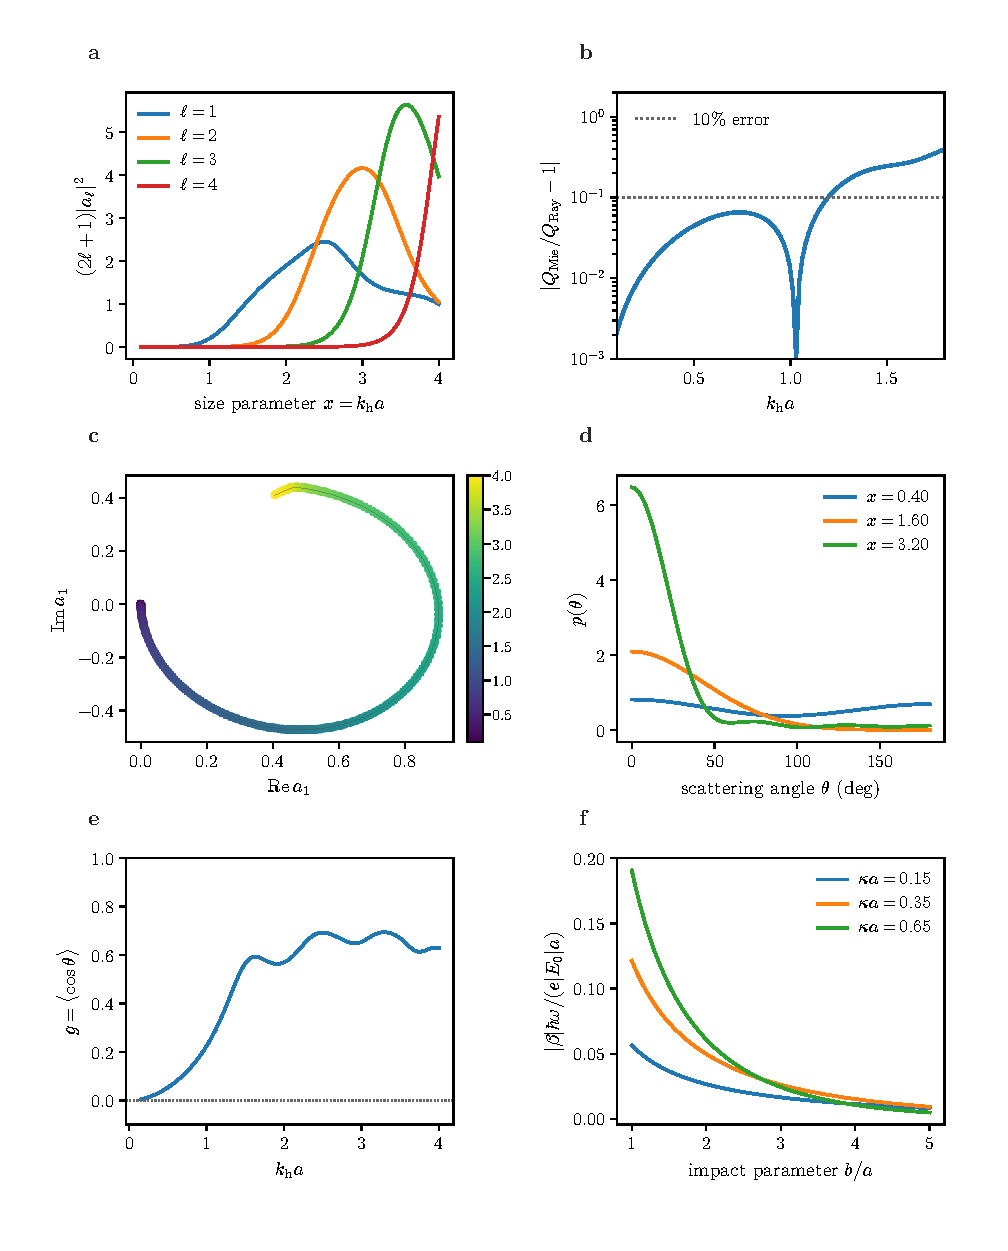
\includegraphics[width=0.96\linewidth,height=0.70\textheight,keepaspectratio]{mie_multipoles_and_electron_sampling.pdf}
\caption{\textbf{球形散射的多极结构与电子轨迹采样。} (a) 各电多极通道 $a_\ell$ 对散射的贡献随尺寸参数 $x=k_{\mathrm h}a$ 增长而依次显现；(b) 精确 Mie 散射效率相对 Rayleigh 近似的误差；(c) 电偶极系数 $a_1$ 的复平面轨迹；(d) 由精确散射振幅得到的角分布从偶极辐射向前向散射转变；(e) 角分布的一阶余弦矩给出方向性；(f) 将球的准静态偶极场代入电子轨迹 Fourier 积分，显示耦合随撞击参数和光学空间频率的衰减。图 (a)--(e) 用完整 Mie 级数，图 (f) 仅在长波准静态层级使用，二者并非在全尺寸范围内采用同一近似。}
\label{fig:mie-multipole-electron}
\end{figure}


半径为 $a$ 的球置于均匀外场 $\vb E_{\rm inc}=E_{\rm L}\hat{\vb x}$。令 $\theta_x$ 为相对极化轴 $x$ 的极角。内外静电势的 $\ell=1$ 解只能写成
\begin{align}
\Phi_{\rm out}
&=-E_{\rm L}r\cos\theta_x+\frac{A\cos\theta_x}{r^2},\\
\Phi_{\rm in}
&=-B E_{\rm L}r\cos\theta_x.
\end{align}
$r=a$ 处切向电场连续等价于电势连续：
\begin{equation}
-E_{\rm L}a+\frac{A}{a^2}=-BE_{\rm L}a.
\label{eq:sphere-bc-general-1}
\end{equation}
法向位移连续给出
\begin{equation}
\varepsilon_{\rm h}
\left(-E_{\rm L}-\frac{2A}{a^3}\right)
=-\varepsilon_{\rm p}BE_{\rm L}.
\label{eq:sphere-bc-general-2}
\end{equation}
由第一式
\(
A=E_{\rm L}a^3(1-B)
\)，代入第二式：
\begin{align}
\varepsilon_{\rm h}\bigl[-1-2(1-B)\bigr]
&=-\varepsilon_{\rm p}B,\\
-3\varepsilon_{\rm h}+2\varepsilon_{\rm h}B
&=-\varepsilon_{\rm p}B,
\end{align}
故
\begin{equation}
B=\frac{3\varepsilon_{\rm h}}{\varepsilon_{\rm p}+2\varepsilon_{\rm h}},
\qquad
A=E_{\rm L}a^3
\frac{\varepsilon_{\rm p}-\varepsilon_{\rm h}}
{\varepsilon_{\rm p}+2\varepsilon_{\rm h}}.
\end{equation}
定义球的无量纲介电对比因子
\begin{equation}
\chi_{\rm sph}(\omega)
\equiv
\frac{\varepsilon_{\rm p}-\varepsilon_{\rm h}}
{\varepsilon_{\rm p}+2\varepsilon_{\rm h}},
\label{eq:chi-sphere-general}
\end{equation}
则偶极矩为
\begin{equation}
{
\vb p
=4\pi\varepsilon_0\varepsilon_{\rm h}a^3
\chi_{\rm sph}\,\vb E_{\rm inc}.}
\label{eq:sphere-polarizability-general}
\end{equation}
真空宿主 $\varepsilon_{\rm h}=1$ 时立即退化为熟悉的 Clausius--Mossotti 球极化率。

为检验准静态边值问题与精确 Maxwell 解的一致性，从 Mie 系数直接作同一个 $x=k_{\rm h}a\ll1$ 展开。以下计算在这里把已经声明的长波条件具体施加到精确 Mie 系数上。

精确 Mie 系数的低阶展开还必须同时检查电偶极与磁偶极通道，不能只凭“粒子很小”预先删除其中一个。
令
$x\ll1$，但此处不再假定 $\mu_{\rm rel}=1$。对 $\ell=1$，最低阶展开为
\begin{align}
\psi_1(x)
&=\frac{x^2}{3}-\frac{x^4}{30}+O(x^6),
&
\psi_1'(x)
&=\frac{2x}{3}-\frac{2x^3}{15}+O(x^5),
\\
\xi_1(x)
&=-\frac{\ii}{x}-\frac{\ii x}{2}
+\frac{x^2}{3}+O(x^3),
&
\xi_1'(x)
&=\frac{\ii}{x^2}-\frac{\ii}{2}
+\frac{2x}{3}+O(x^2).
\end{align}
对 electric/TM 系数，分子最低阶为
\begin{align}
N_1^{(E)}
&=m_{\rm r}\psi_1(m_{\rm r}x)\psi_1'(x)
-\mu_{\rm rel}\psi_1(x)\psi_1'(m_{\rm r}x)
\\
&=m_{\rm r}
\left(\frac{m_{\rm r}^2x^2}{3}\right)
\left(\frac{2x}{3}\right)
-\mu_{\rm rel}
\left(\frac{x^2}{3}\right)
\left(\frac{2m_{\rm r}x}{3}\right)
+O(x^5)
\\
&=\frac{2m_{\rm r}\mu_{\rm rel}}{9}
(\varepsilon_{\rm rel}-1)x^3+O(x^5),
\end{align}
因为 $m_{\rm r}^2=\varepsilon_{\rm rel}\mu_{\rm rel}$。分母最低阶为
\begin{align}
D_1^{(E)}
&=m_{\rm r}\psi_1(m_{\rm r}x)\xi_1'(x)
-\mu_{\rm rel}\xi_1(x)\psi_1'(m_{\rm r}x)
\\
&=m_{\rm r}
\left(\frac{m_{\rm r}^2x^2}{3}\right)
\frac{\ii}{x^2}
-\mu_{\rm rel}
\left(-\frac{\ii}{x}\right)
\left(\frac{2m_{\rm r}x}{3}\right)
+O(x^2)
\\
&=\frac{\ii m_{\rm r}\mu_{\rm rel}}{3}
(\varepsilon_{\rm rel}+2)+O(x^2).
\end{align}
所以
\begin{equation}
{
a_1
=-\frac{2\ii}{3}
\frac{\varepsilon_{\rm rel}-1}
{\varepsilon_{\rm rel}+2}x^3
+O(x^5).}
\label{eq:mie-rayleigh-a-general}
\end{equation}
magnetic/TE 通道也必须逐项展开。由式~\cref{eq:mie-b-standard}，其分子为
\begin{align}
N_1^{(M)}
&=\mu_{\rm rel}\psi_1(m_{\rm r}x)\psi_1'(x)
-m_{\rm r}\psi_1(x)\psi_1'(m_{\rm r}x)\\
&=\mu_{\rm rel}
\left(\frac{m_{\rm r}^2x^2}{3}\right)
\left(\frac{2x}{3}\right)
-m_{\rm r}
\left(\frac{x^2}{3}\right)
\left(\frac{2m_{\rm r}x}{3}\right)
+O(x^5)\\
&=\frac{2m_{\rm r}^2}{9}(\mu_{\rm rel}-1)x^3+O(x^5).
\end{align}
分母为
\begin{align}
D_1^{(M)}
&=\mu_{\rm rel}\psi_1(m_{\rm r}x)\xi_1'(x)
-m_{\rm r}\xi_1(x)\psi_1'(m_{\rm r}x)\\
&=\mu_{\rm rel}
\left(\frac{m_{\rm r}^2x^2}{3}\right)
\frac{\ii}{x^2}
-m_{\rm r}
\left(-\frac{\ii}{x}\right)
\left(\frac{2m_{\rm r}x}{3}\right)
+O(x^2)\\
&=\frac{\ii m_{\rm r}^2}{3}(\mu_{\rm rel}+2)+O(x^2).
\end{align}
于是
\begin{equation}
{
b_1
=-\frac{2\ii}{3}
\frac{\mu_{\rm rel}-1}
{\mu_{\rm rel}+2}x^3
+O(x^5).}
\label{eq:mie-rayleigh-b-general}
\end{equation}
这表明一般磁介质在 Rayleigh 阶就有独立磁偶极响应。只有在非磁性特例 $\mu_{\rm rel}=1$ 时，分子中的 $x^3$ 项严格相消，因此必须把 $\psi_1,\psi_1'$ 多保留两阶：
\begin{align}
\psi_1(z)&=\frac{z^2}{3}-\frac{z^4}{30}+O(z^6),\\
\psi_1'(z)&=\frac{2z}{3}-\frac{2z^3}{15}+O(z^5).
\end{align}
于是
\begin{align}
\psi_1(m_{\rm r}x)\psi_1'(x)
&=\frac{2m_{\rm r}^2}{9}x^3
-\frac{2m_{\rm r}^2+m_{\rm r}^4}{45}x^5+O(x^7),\\
m_{\rm r}\psi_1(x)\psi_1'(m_{\rm r}x)
&=\frac{2m_{\rm r}^2}{9}x^3
-\frac{m_{\rm r}^2+2m_{\rm r}^4}{45}x^5+O(x^7).
\end{align}
两式相减，$x^3$ 项完全抵消，留下
\begin{equation}
N_1^{(M)}\big|_{\mu_{\rm rel}=1}
=\frac{m_{\rm r}^2(m_{\rm r}^2-1)}{45}x^5+O(x^7).
\end{equation}
而分母只需最低阶
\begin{equation}
D_1^{(M)}\big|_{\mu_{\rm rel}=1}
=\ii m_{\rm r}^2+O(x^2).
\end{equation}
故
\begin{equation}
{
b_1
=-\frac{\ii}{45}
(m_{\rm r}^2-1)x^5+O(x^7),
\qquad
\mu_{\rm rel}=1.}
\label{eq:mie-rayleigh-b-nonmagnetic}
\end{equation}
此时式~\cref{eq:mie-rayleigh-a-general} 又化为
\begin{equation}
a_1
=-\frac{2\ii}{3}
\frac{m_{\rm r}^2-1}{m_{\rm r}^2+2}x^3+O(x^5),
\end{equation}
其中材料因子正是式~\cref{eq:chi-sphere-general} 的
$\chi_{\rm sph}$。因此 quasistatic 电偶极结果就是完整 Mie electric/TM $\ell=1$ 通道的最低阶。


在 quasistatic 区，宿主中的散射近场是
\begin{equation}
\vb E_{\rm sc}(\vb r)
=E_{\rm L}\chi_{\rm sph}a^3
\frac{3\hat{\vb r}(\hat{\vb r}\cdot\hat{\vb x})-\hat{\vb x}}{r^3}.
\label{eq:sphere-quasistatic-field}
\end{equation}
取电子沿 $z$ 传播，横向位置写成
\begin{equation}
x=b\cos\varphi,
\qquad
y=b\sin\varphi,
\qquad r^2=b^2+z^2.
\end{equation}
于是电子真正耦合的纵向场为
\begin{equation}
E_{\omega,z}^{(\rm sph)}(b,\varphi,z)
=3E_{\rm L}\chi_{\rm sph}a^3
\frac{b\cos\varphi\,z}{(b^2+z^2)^{5/2}}.
\label{eq:Ez-sphere-general}
\end{equation}
定义电子相位匹配波数
\begin{equation}
\kappa\equiv\frac{\omega}{v_0}>0.
\label{eq:kappa-electron}
\end{equation}
利用
\begin{equation}
\frac{3z}{(b^2+z^2)^{5/2}}
=-\frac{\dd}{\dd z}(b^2+z^2)^{-3/2}
\end{equation}
并分部积分，边界项在 $|z|\to\infty$ 消失：
\begin{align}
\mathcal F_{\parallel}^{(\rm sph)}
&=E_{\rm L}\chi_{\rm sph}a^3b\cos\varphi
\int_{-\infty}^{+\infty}\!\dd z\,
\frac{3z}{(b^2+z^2)^{5/2}}\ee^{-\ii\kappa z}\\
&=-\ii\kappa E_{\rm L}\chi_{\rm sph}a^3b\cos\varphi
\int_{-\infty}^{+\infty}\!\dd z\,
\frac{\ee^{-\ii\kappa z}}{(b^2+z^2)^{3/2}}.
\end{align}
剩余 Fourier 积分可以用 Schwinger 参数化逐步算出。对 $b>0$，有
\begin{equation}
\frac{1}{(b^2+z^2)^{3/2}}
=\frac{1}{\Gamma(3/2)}
\int_0^{\infty} t^{1/2}\ee^{-t(b^2+z^2)}\dd t
=\frac{2}{\sqrt\pi}
\int_0^{\infty} t^{1/2}\ee^{-t(b^2+z^2)}\dd t.
\label{eq:schwinger-three-halves}
\end{equation}
因为左端关于 $z$ 绝对可积，交换 $z$、$t$ 积分是合法的。于是
\begin{align}
I_{3/2}(b,\kappa)
&\equiv
\int_{-\infty}^{+\infty}
\frac{\ee^{-\ii\kappa z}}{(b^2+z^2)^{3/2}}\dd z\\
&=\frac{2}{\sqrt\pi}
\int_0^{\infty}t^{1/2}\ee^{-b^2t}
\left[
\int_{-\infty}^{+\infty}
\ee^{-tz^2-\ii\kappa z}\dd z
\right]\dd t.
\end{align}
内层是标准 Gaussian Fourier 积分。配方
\begin{equation}
-tz^2-\ii\kappa z
=-t\left(z+\frac{\ii\kappa}{2t}\right)^2
-\frac{\kappa^2}{4t},
\end{equation}
故
\begin{equation}
\int_{-\infty}^{+\infty}
\ee^{-tz^2-\ii\kappa z}\dd z
=\sqrt{\frac{\pi}{t}}
\exp\!\left(-\frac{\kappa^2}{4t}\right).
\end{equation}
因此
\begin{align}
I_{3/2}
&=2\int_0^{\infty}
\exp\!\left(-b^2t-\frac{\kappa^2}{4t}\right)\dd t.
\end{align}
再令 $u=b^2t$，则
\begin{align}
I_{3/2}
&=\frac{2}{b^2}
\int_0^{\infty}
\exp\!\left[-u-\frac{(\kappa b)^2}{4u}\right]\dd u.
\end{align}
使用修正 Bessel 函数的积分表示
\begin{equation}
K_\nu(x)
=\frac12\left(\frac{x}{2}\right)^\nu
\int_0^{\infty}u^{-\nu-1}
\exp\!\left(-u-\frac{x^2}{4u}\right)\dd u,
\end{equation}
并取 $\nu=-1$，再用 $K_{-1}=K_1$，得到
\begin{equation}
\int_0^{\infty}
\exp\!\left(-u-\frac{x^2}{4u}\right)\dd u
=xK_1(x).
\end{equation}
所以
\begin{equation}
{
\int_{-\infty}^{+\infty}
\frac{\ee^{-\ii\kappa z}}{(b^2+z^2)^{3/2}}\dd z
=\frac{2\kappa}{b}K_1(\kappa b).}
\label{eq:K1-trajectory-transform}
\end{equation}
代回上式得到
\begin{equation}
{
\mathcal F_{\parallel}^{(\rm sph)}(b,\varphi)
=-2\ii E_{\rm L}\chi_{\rm sph}a^3
\kappa^2K_1(\kappa b)\cos\varphi.}
\label{eq:F-sphere-general}
\end{equation}
当 $\kappa b\ll1$ 时 $K_1(x)=x^{-1}+O(x\ln x)$，所以
\begin{equation}
|\mathcal F_{\parallel}^{(\rm sph)}|
\simeq
2|E_{\rm L}\chi_{\rm sph}|a^3
\frac{\kappa}{b}|\cos\varphi|.
\label{eq:F-sphere-small-kappa}
\end{equation}
若实验主要采样 $b\sim a$，则 $|\mathcal F_{\parallel}|\propto a^2$。


以上的 $K_1$ 结果已经从球面边界条件和 Fourier 积分完整得到。它只描述诱导偶极垂直于电子轨迹、且其横向投影正好指向撞击参数的情形。实验可以转动照明偏振，也可以改变电子在球周围的方位角；此时只沿用 $K_1$ 会遗漏纵向偶极造成的另一条相干路径。需要回到同一个偶极势，并在进行能量通道求和之前保留所有复振幅。

取真空宿主、非磁性球，沿用前面定义的 $\chi_{\rm sph}$。在长波近似下诱导偶极矩的任意笛卡儿分量由同一个复极化率给出：
\begin{equation}
\vb p=4\pi\varepsilon_0a^3\chi_{\rm sph}\,\vb E_{\rm inc}.
\label{eq:sphere-dipole-worked}
\end{equation}
这里 $\vb E_{\rm inc}$ 是完整复相量，而不是正频率解析信号的半振幅。设电子沿 $+z$ 方向通过球外，撞击参数为 $b>a$，方位角为 $\varphi$，并把偶极矩的横向投影记为 $p_b=p_x\cos\varphi+p_y\sin\varphi$。沿轨迹 $\vb r=(b\cos\varphi,b\sin\varphi,z)$，散射场的标势为
\begin{equation}
\Phi_{\rm dip}(b,\varphi,z)
=\frac{p_b b+p_z z}{4\pi\varepsilon_0(b^2+z^2)^{3/2}}.
\label{eq:dipole-general-potential}
\end{equation}
由 $E_{\omega,z}^{\rm dip}=-\partial_z\Phi_{\rm dip}$ 得
\begin{align}
E_{\omega,z}^{\rm dip}
&=\frac{3p_b b z+p_z(2z^2-b^2)}
{4\pi\varepsilon_0(b^2+z^2)^{5/2}},
\label{eq:dipole-trajectory-field}\\
\mathcal F_\parallel
&=-\ii\kappa\int_{-\infty}^{\infty}\Phi_{\rm dip}
\ee^{-\ii\kappa z}\dd z,\qquad \kappa=\omega/v_0>0.
\end{align}
第二行对 $-\partial_z\Phi$ 分部积分，边界项因 $\Phi\to0$ 而消失。可见横向分量关于 $z$ 为奇函数，纵向分量关于 $z$ 为偶函数；即使两种入射偶极的复振幅相同，轨迹 Fourier 投影也会相差四分之一个周期的相位。

横向偶极需要的积分已由\cref{eq:K1-trajectory-transform} 给出，直接乘以 $b$ 即为 $2\kappa K_1(\kappa b)$。纵向分量则涉及
\begin{equation*}
I_z(b,\kappa)=\int_{-\infty}^{\infty}
\frac{z\,\ee^{-\ii\kappa z}}{(b^2+z^2)^{3/2}}\dd z.
\end{equation*}
为求这条积分，不必重新进行 Schwinger 参数化。记
\begin{equation*}
G_0(b,\kappa)=\int_{-\infty}^{\infty}
\frac{\ee^{-\ii\kappa z}}{\sqrt{b^2+z^2}}\dd z.
\end{equation*}
该振荡积分可按对称截断后的极限理解；在 $\kappa>0$ 下，先对 $b$ 微分并使用前面已经收敛的积分，得到
\begin{align*}
\frac{\partial G_0}{\partial b}
&=-b\int_{-\infty}^{\infty}
\frac{\ee^{-\ii\kappa z}}{(b^2+z^2)^{3/2}}\dd z
=-2\kappa K_1(\kappa b),\\
G_0(b,\kappa)&=2K_0(\kappa b).
\end{align*}
最后的积分常数由固定 $\kappa>0$ 时 $b\to\infty$ 的振荡积分趋零确定。因为
$z/(b^2+z^2)^{3/2}=-\partial_z(b^2+z^2)^{-1/2}$，再做一次分部积分便得到
\begin{equation}
I_z(b,\kappa)=-\ii\kappa G_0(b,\kappa)
=-2\ii\kappa K_0(\kappa b).
\label{eq:rayleigh-K0-longitudinal-transform}
\end{equation}
把横向和纵向两条积分代回同一个 $\mathcal F_\parallel$，先相加复振幅、再乘以电子耦合的公共因子，得到
\begin{equation}
\begin{aligned}
\mathcal F_\parallel(b,\varphi)
&=-\frac{\kappa^2}{2\pi\varepsilon_0}
\left[\ii p_bK_1(\kappa b)+p_zK_0(\kappa b)\right],\\
\beta(b,\varphi)
&=-\frac{e\kappa^2}{4\pi\varepsilon_0\hbar\omega}
\left[\ii p_bK_1(\kappa b)+p_zK_0(\kappa b)\right].
\end{aligned}
\label{eq:rayleigh-polarization-projection}
\end{equation}
将 $p_z=0$、$p_b=p$ 代入，恢复单独横向偶极的结果
\begin{equation}
\beta_\perp(b)=-\frac{\ii e p\kappa^2}{4\pi\varepsilon_0\hbar\omega}K_1(\kappa b).
\label{eq:dipole-to-beta-worked}
\end{equation}
它与\cref{eq:F-sphere-general} 完全一致。相反，$p_b=0$ 时只留下实的 $K_0$ 投影（若 $p_z$ 为实）；不同偏振通道并不是仅仅改变同一张耦合图的高度。

为了看清相位干涉，令 $p_b=p_0\cos\theta$，$p_z=p_0\sin\theta\ee^{\ii\delta}$。这里 $\theta$ 调节两种偶极分量的权重，$\delta$ 是它们的相对光学相位，并不等同于电子能量阶数。于是
\begin{equation}
\beta=-\frac{e\kappa^2p_0}{4\pi\varepsilon_0\hbar\omega}
\left[\ii\cos\theta\,K_1(\kappa b)
+\sin\theta\ee^{\ii\delta}K_0(\kappa b)\right].
\label{eq:rayleigh-polarization-null}
\end{equation}
在给定 $b$ 处，两个投影发生严格相消的条件为
\begin{equation}
\delta=-\frac\pi2,\qquad
\tan\theta=\frac{K_1(\kappa b)}{K_0(\kappa b)}.
\label{eq:rayleigh-polarization-cancel-condition}
\end{equation}
这不是球的材料共振消失，而是电子所选的纵向 Fourier 分量相消。若把轨迹转到球的另一侧，$p_b$ 改变符号，而 $p_z$ 不变；于是椭圆偏振的两个复投影可以构成空间上的左右不对称能量滤波像。只有在相位参考固定、实验保持两种偏振的相干性时，这一干涉才会出现。它仍属于准静态球和直线电子轨迹的理论预测，不能直接用于 $k_0a\gtrsim1$ 或强电子偏折的情形。

在更一般的电子轨迹方位角 $\varphi$ 上，横向偶极必须先投影到撞击参数方向，因而 $p_b=p_0\cos\theta\cos\varphi$。令
\[
 B=-\frac{e\kappa^2p_0}{4\pi\varepsilon_0\hbar\omega},\qquad
 t=K_1(\kappa b),\quad u=K_0(\kappa b),
\]
则同一个复耦合可写为
\begin{equation}
 \beta_\delta(b,\theta,\varphi)=
 B\left[\ii t\cos\theta\cos\varphi
 +u\sin\theta\ee^{\ii\delta}\right].
 \label{eq:rayleigh-azimuthal-polarization}
\end{equation}
这是理解空间成像与相位消光所需的完整参数依赖。横向通道乘以 $\cos\varphi$，因此电子绕球转到另一侧时该通道变号；纵向通道不变号。除了耦合模长，还应追踪复数 $\beta$ 在复平面内随 $\delta$ 的轨迹：它是一条以 $\ii Bt\cos\theta\cos\varphi$ 为圆心、以 $|B|u\sin\theta$ 为半径的圆。当圆经过原点时，特定电子轨迹的全部非零阶边带同时消失。

\begin{figure}[!htbp]
\centering
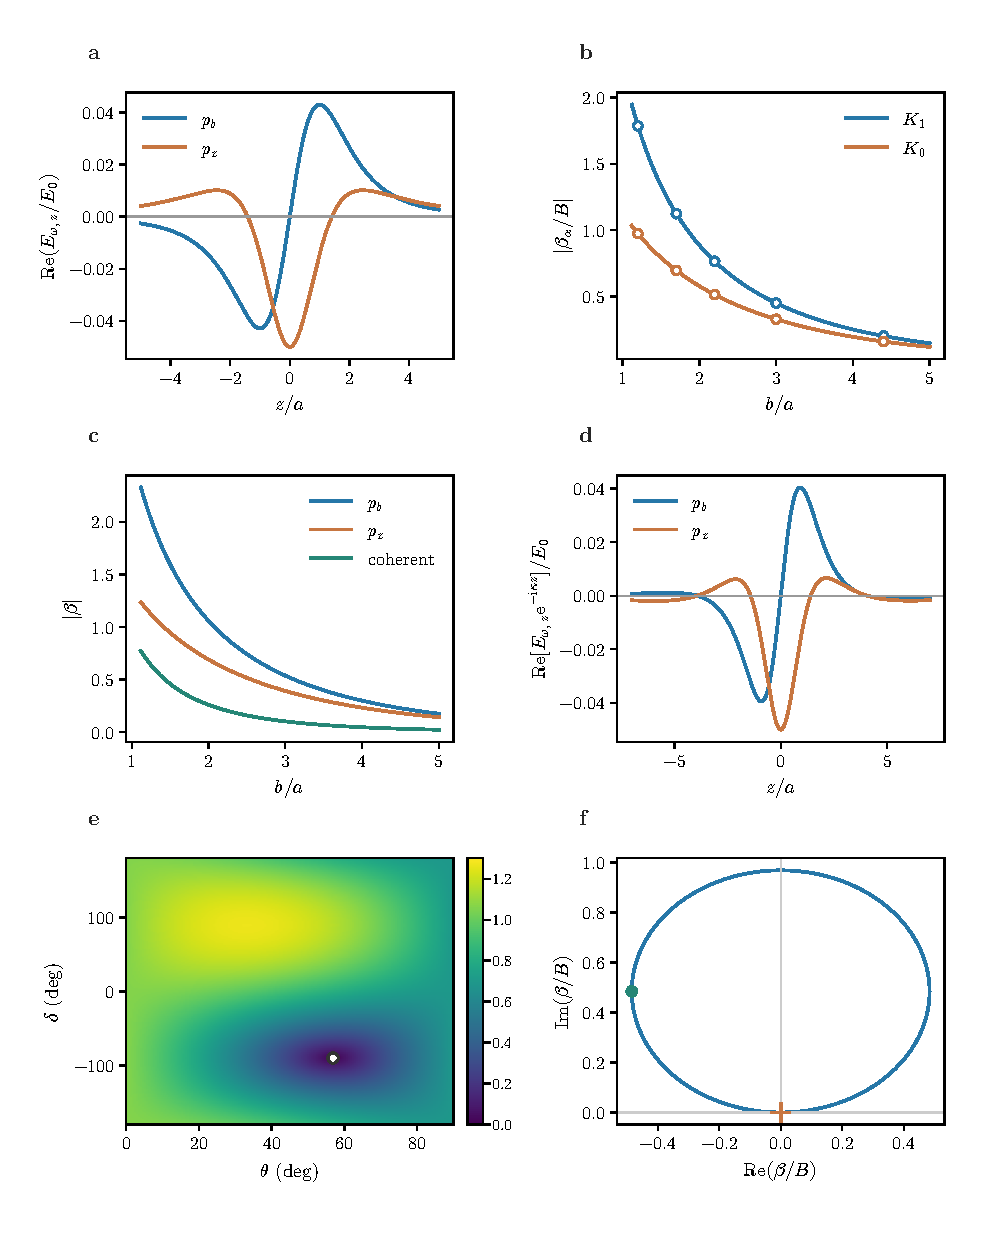
\includegraphics[width=0.98\linewidth,height=0.57\textheight,keepaspectratio]{polarization_resolved_rayleigh.pdf}
\caption{\textbf{Rayleigh 球的两种偶极 Fourier 投影及复耦合。}
(a) 横向 $p_b$ 与纵向 $p_z$ 偶极在 $b=2a$ 的有符号纵向电场；
(b) $K_1$ 与 $K_0$ 核函数，空心圆由独立轨迹积分给出；
(c) 两条通道及其相干叠加随撞击参数改变的 $|\beta|$；
(d) 乘上电子相位因子 $\ee^{-\ii\kappa z}$ 后的 Fourier 被积函数实部；
(e) 双参数 $\theta,\delta$ 下的耦合模长，白点满足解析相消条件；
(f) 相位 $\delta$ 绕行一周时，归一化复振幅 $\beta/B$ 在复平面中的圆轨迹，橙色叉号为零耦合点。面板 (a)--(f) 的曲线来自同一个有符号准静态偶极场。}
\label{fig:rayleigh-polarization-selectivity}
\end{figure}

读图时尤其需要区分两种不同的零点。图 (a) 和图 (d) 中，电场或 Fourier 被积函数可以在某个 $z$ 变号，但单独一处变号并不意味着积分为零。图 (e) 和图 (f) 的相消则发生在\emph{完成整个轨迹积分之后}：两种正交偶极的复投影恰好反向，所以相干和为零。这使偏振角成为可以在没有改变颗粒本征响应的情况下关闭特定电子散射通道的控制量。

接下来需要问的是，这种复振幅零点在仪器中到底表现为何种能量谱。对经典单色相干近场，同一个 $|\beta|$ 决定所有能量交换通道；利用 $J_{-n}(x)=(-1)^nJ_n(x)$，直接得到
\begin{equation}
 P_{+n}(\delta)=P_{-n}(\delta)=J_n^2\bigl(2|\beta_\delta|\bigr),\qquad
 I_{\mathrm{inel}}=1-P_0=1-J_0^2\bigl(2|\beta_\delta|\bigr).
 \label{eq:rayleigh-polarization-sidebands}
\end{equation}
因此，改变照明椭圆偏振的手性，能够交换球左右两侧的\emph{非弹性成像对比}，却不会仅凭这一经典相干模型导致同一轨迹的电子增益、损失概率不对称。后一种不对称若在实验中出现，必须检查入射电子态、量子光子数分布或其他超出本模型的动力学。

两种相反手性 $\delta=\pm\pi/2$ 所产生的干涉差别可以直接由\cref{eq:rayleigh-azimuthal-polarization} 算出。设 $C=t\cos\theta\cos\varphi$，$D=u\sin\theta$，则 $\beta_\pm=\ii B(C\pm D)$，从而
\begin{equation}
 |\beta_+|^2-|\beta_-|^2
 =4|B|^2K_1(\kappa b)K_0(\kappa b)
 \cos\theta\sin\theta\cos\varphi.
 \label{eq:rayleigh-polarization-handedness}
\end{equation}
式右侧对 $\varphi\mapsto\varphi+\pi$ 变号：两种照明手性使左右两侧互换明暗，但不改变能量阶数 $n$ 的正负对称性。为避免对比图混入总光强变化，定义两个手性下的电子非弹性信号 $I_\pm=1-J_0^2(2|\beta_\pm|)$，并取
\begin{equation}
 \mathcal A(\theta,\varphi)=\frac{I_+-I_-}{I_++I_-},
 \label{eq:rayleigh-polarization-asymmetry}
\end{equation}
在 $I_++I_-=0$ 的点约定 $\mathcal A=0$。因为 $J_0^2$ 对其自变量并非单调函数，$\mathcal A$ 不能未经前向拟合就等同于\cref{eq:rayleigh-polarization-handedness} 的二次耦合差。

严格消光点对偏振角误差的敏感程度也可以从解析式得出。令 $\theta_0=\arctan(t/u)$、$\theta=\theta_0+\Delta\theta$、$\delta=-\pi/2+\Delta\delta$，在 $\varphi=0$ 处对两个小偏移展开：
\begin{align*}
 \frac{\beta}{B}
 &=\ii\bigl(t\cos\theta-u\sin\theta\bigr)
 +u\sin\theta\bigl(\ee^{\ii\Delta\delta}-1\bigr)(-\ii)\\
 &=-\ii\sqrt{t^2+u^2}\,\Delta\theta
 +\frac{tu}{\sqrt{t^2+u^2}}\,\Delta\delta
 +O(\Delta\theta^2,\Delta\delta^2,\Delta\theta\Delta\delta).
\end{align*}
于是首个非零的消光附近强度为
\begin{equation}
 |\beta|^2=|B|^2\left[(t^2+u^2)(\Delta\theta)^2
 +\frac{t^2u^2}{t^2+u^2}(\Delta\delta)^2\right]
 +O(\|\Delta\|^3).
 \label{eq:rayleigh-polarization-null-curvature}
\end{equation}
这说明消光点附近的双参数灵敏度是各向异性的：混合角误差和相对相位误差沿不同正交方向打开耦合，而不是产生一个通用的“偏振误差百分比”。

\begin{figure}[!htbp]
\centering
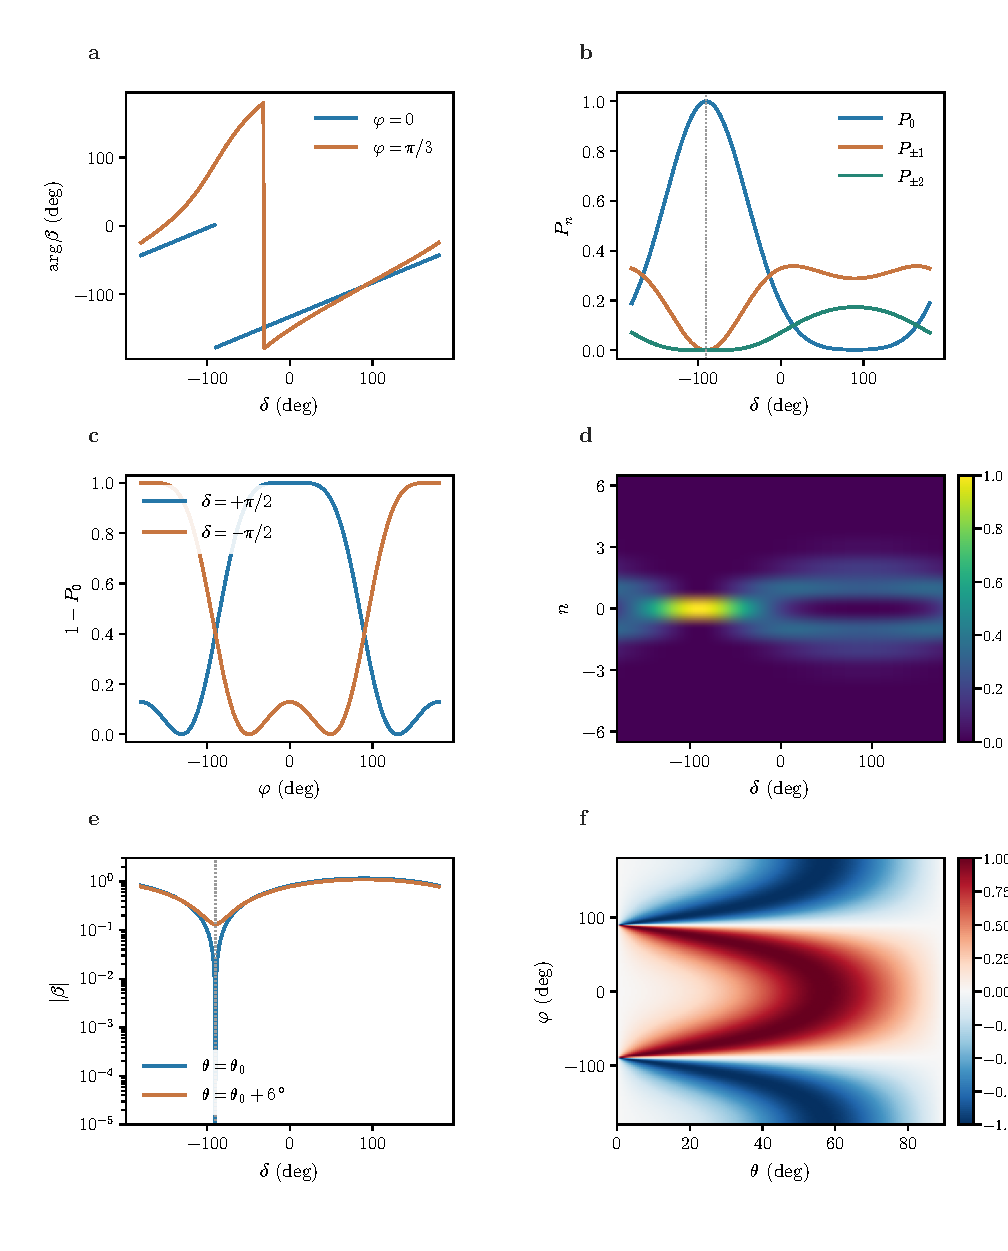
\includegraphics[width=0.98\linewidth,height=0.57\textheight,keepaspectratio]{polarization_resolved_spectroscopy.pdf}
\caption{\textbf{从偏振相干控制到 PINEM 边带与电子成像。}
(a) 两条轨迹方位上的复耦合相位 $\arg\beta$，主值相位的 $\pm180^\circ$ 跳变只是分支切换；
(b) 消光角处的 $P_0$、$P_{\pm1}$、$P_{\pm2}$，正负交换阶精确重合；
(c) 两种相反偏振手性产生的非弹性成像对比 $1-P_0$；
(d) 完整增益--损失能量阶梯随相对相位变化的概率分布；
(e) 消光点附近偏离混合角 $6^\circ$ 所造成的有限耦合底；
(f) 由两个手性电子信号构造的归一化空间非对称度 $\mathcal A$。该图是单电子、单色经典相干场的概率预测。}
\label{fig:rayleigh-polarization-spectroscopy}
\end{figure}

两组六联图采用相同的 $a=30\,\mathrm{nm}$、$\lambda=800\,\mathrm{nm}$、$v_0=0.60c$、$E_0=10^9\,\mathrm{V/m}$、真空背景与频率无关的唯象介电常数 $\varepsilon_r=3+0.10\ii$。极化率取 $p_0=4\pi\varepsilon_0a^3(\varepsilon_r-1)/(\varepsilon_r+2)E_0$，因而 $B$ 在整组计算中不再额外拟合；$\kappa=\omega/v_0$、$b_0=2a$。它们只用于展示准静态 Rayleigh 球，不代表任何真实材料的实验色散参数。

\cref{fig:rayleigh-polarization-selectivity} 的 (a) 为 $z/a\in[-5,5]$ 的 501 点、$b=b_0$ 的 $\operatorname{Re}(E_{\omega,z}/E_0)$；(b) 为 $b/a\in[1.12,5.0]$ 的 110 点的 $K_1,K_0$，空心点在 $b/a=1.2,1.7,2.2,3.0,4.4$ 用 $z/a\in[-350,350]$ 的 20001 点 Simpson 积分检查；(c) 比较两单独偶极与 $\theta=\pi/4,\delta=-\pi/2$ 的相干叠加；(d) 为 $z/a\in[-7,7]$ 的 701 点上 Fourier 被积函数实部；(e) 为 $\theta\in[0,\pi/2]$ 的 161 点、$\delta\in[-\pi,\pi]$ 的 241 点的 $|\beta|$；(f) 为 $\theta=\theta_0,\varphi=0$、在 $[-\pi,\pi]$ 的 501 个相位点上画出的 $\beta/B$ 复平面轨迹。解析相消发生在 $\theta_0=\arctan[K_1(\kappa b_0)/K_0(\kappa b_0)]$ 与 $\delta=-\pi/2$。

\cref{fig:rayleigh-polarization-spectroscopy} 的 (a) 使用 $\theta=\theta_0$、$\varphi=0,\pi/3$，取 361 个 $\delta\in[-\pi,\pi]$ 点，并将 $|\beta|<10^{-9}$ 的相位设为未定义；(b) 固定 $\varphi=0$，用同一 361 点计算 $P_0$、$J_1^2(2|\beta|)$、$J_2^2(2|\beta|)$；(c) 固定 $\theta=\pi/4$，在 361 个 $\varphi\in[-\pi,\pi]$ 点比较 $\delta=\pm\pi/2$ 的 $1-P_0$；(d) 用 $n=-6,\ldots,6$ 的贝塞尔阶数计算随 $\delta$ 的联合概率热图，不对有限阶窗口再次归一化；(e) 比较 $\theta=\theta_0$ 与 $\theta_0+6^\circ$ 的 $|\beta|$，对数图的可视化下限为 $10^{-5}$，不改变原始计算数据；(f) 用 $\theta\in[0,\pi/2]$ 的 161 点、$\varphi\in[-\pi,\pi]$ 的 271 点，按\cref{eq:rayleigh-polarization-asymmetry} 计算双手性电子图像。全部计算使用理想单次电子概率，不含探测器模糊、未分辨偏振平均、退相干或束流空间平均。

将这一 $\beta(b)$ 代回已经推导出的电子响应，可以直接得到撞击参数依赖的离散能谱
\begin{equation}
 P_n(b)=J_n^2\!\left(2|\beta(b)|\right),
 \qquad \sum_{n=-\infty}^{\infty}P_n(b)=1.
 \label{eq:dipole-spectrum-worked}
\end{equation}
假设探测器的能量响应为归一化的高斯函数
$G_{\sigma_E}(\mathcal E)=(2\pi\sigma_E^2)^{-1/2}
\ee^{-\mathcal E^2/(2\sigma_E^2)}$，则真实记录的连续能损密度为
\begin{equation}
 I(\Delta\mathcal E\mid b)=
 \sum_{n=-\infty}^{\infty}P_n(b)
 G_{\sigma_E}(\Delta\mathcal E-n\hbar\omega).
 \label{eq:dipole-detector-worked}
\end{equation}
此处没有背景和效率损失；若引入背景或有限计数，应该在这一归一化谱之后另用探测器前向模型处理。高斯响应的积分为一，因而 $\int\dd(\Delta\mathcal E)I=1$。这就从球形边值问题一直推到了能量谱，而没有在中间人为指定 $\beta(b)$ 的形状。

\begin{figure}[!htbp]
 \centering
 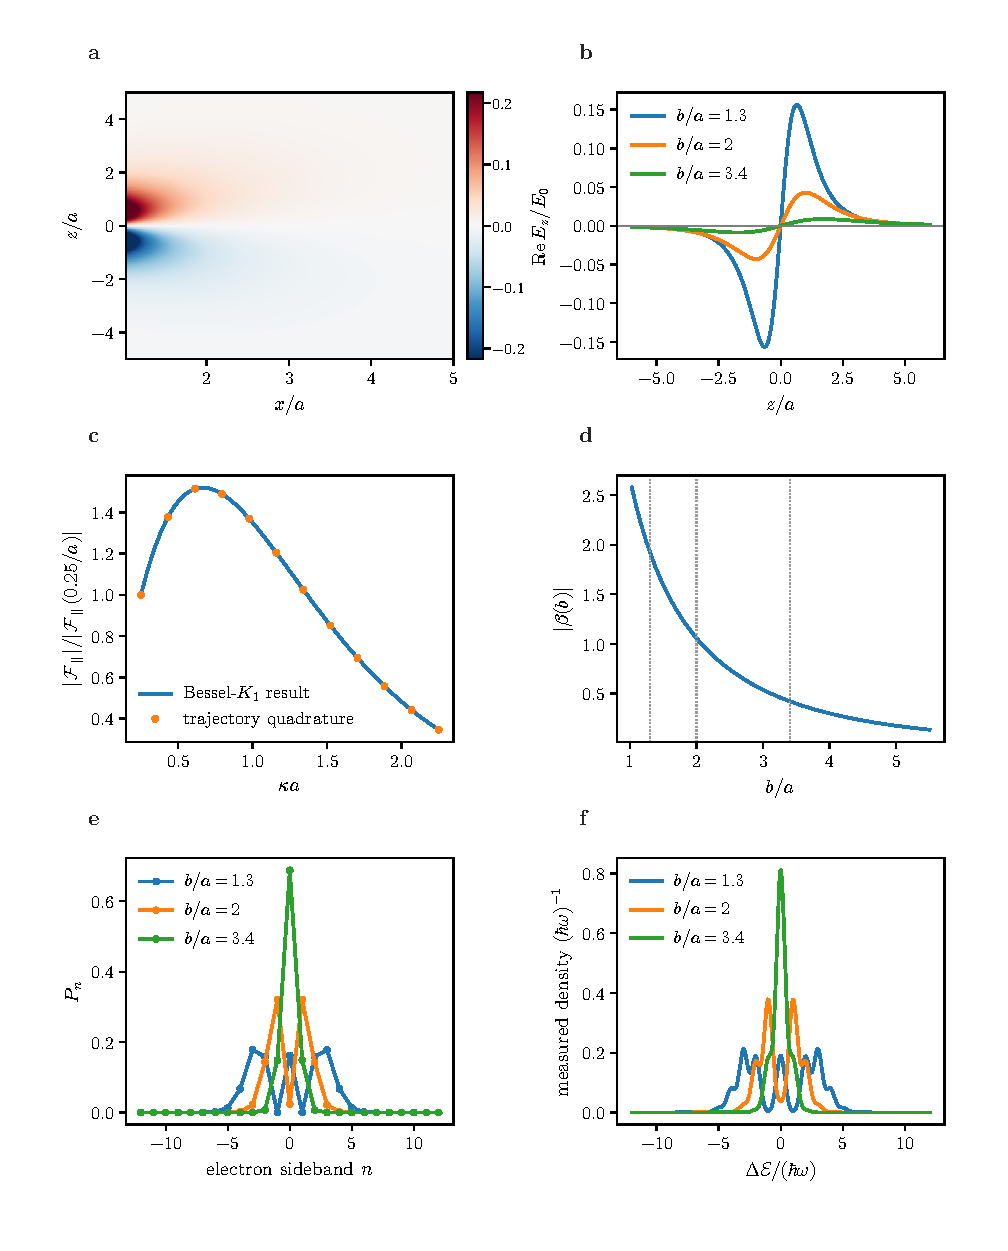
\includegraphics[width=0.98\linewidth,height=0.70\textheight,keepaspectratio]{dipole_to_measured_spectrum.pdf}
 \caption{\textbf{从球形近场到实际电子能谱的连续计算。}
 (a) 介质偶极沿电子轨迹方向的有符号电场；(b) 三个撞击参数处的纵向场截面；
 (c) 修正贝塞尔函数解析结果与直接轨迹求积的对照；(d) 撞击参数变化时的复耦合模；
 (e) 同一耦合参数给出的贝塞尔边带人口；(f) 经过有限能量分辨率卷积后的实际能谱。
 所有面板来自\cref{eq:dipole-trajectory-field,eq:dipole-to-beta-worked,eq:dipole-spectrum-worked,eq:dipole-detector-worked}，不是独立拟合曲线。}
 \label{fig:dipole-to-measured-spectrum}
\end{figure}

为了复算这六幅图，固定 $a=30\,\mathrm{nm}$、$\lambda=800\,\mathrm{nm}$、$v_0=0.60c$、
$E_0=1.0\times10^9\,\mathrm{V/m}$，真空宿主及频率无关的唯象介电常数
$\varepsilon_r=3.0+0.10\ii$。这些数字只用于构造具有可见多边带的教学算例，特别是材料色散、空间非均匀激光驱动和束斑平均尚未包含。
图 (a) 使用 $x/a\in[1.02,5]$ 的 215 点及 $z/a\in[-5,5]$ 的 260 点；图 (b) 对
$b/a=1.3,2.0,3.4$ 绘制 $z/a\in[-6,6]$ 的 560 点。
图 (c) 固定 $b/a=2$，取 $\kappa a\in[0.25,2.25]$ 共 45 点，直接求积使用 $z/a\in[-300,300]$ 的 22001 点 Simpson 网格；图 (d) 取 $b/a\in[1.03,5.5]$ 共 320 点。图 (e) 截断到 $|n|\le12$，图 (f) 截断到 $|n|\le22$，高斯宽度 $\sigma_E/(\hbar\omega)=0.34$，绘制 $\Delta\mathcal E/(\hbar\omega)\in[-12,12]$ 共 700 点，谱线没有再作峰值归一化。图 (c) 中的归一化仅为便于比较不同 $\kappa$ 时的曲线形状，其他面板各自采用式中给出的量纲或概率归一化。

这一算例给出了一条可以迁移到非球形纳米结构的方法：改变材料或几何，只需重求 $\vb E_\omega$；电子侧的轨迹积分、贝塞尔概率和探测器卷积保持相同的数学层级。失效的地方也可以逐个定位：$k_0a\not\ll1$ 时要回到精确 Mie 多极场，显著反冲时要回到有限通道动力学，而束斑有限时应在强度层面对 $b$ 的分布积分，不能先将不同轨迹的复 $\beta$ 简单平均。


在均匀宿主 $\varepsilon_{\rm h}(\omega)$ 中，第一个独立控制量来自材料本身。对于本章正文保留的球几何，它就是式~\cref{eq:chi-sphere-general} 已经由准静态边值问题和 Mie 渐近共同导出的
\begin{equation}
{
\chi_{\rm sph}(\omega)
=\frac{\varepsilon_{\rm p}(\omega)-\varepsilon_{\rm h}(\omega)}
{\varepsilon_{\rm p}(\omega)+2\varepsilon_{\rm h}(\omega)}.}
\label{eq:material-contrast-factors}
\end{equation}
因此准静态电偶极增强首先受分母
$\varepsilon_{\rm p}+2\varepsilon_{\rm h}$ 控制。若损耗有限而且实部可以穿过零点，则共振附近满足
\begin{equation}
\operatorname{Re}\!\left[\varepsilon_{\rm p}(\omega)+2\varepsilon_{\rm h}(\omega)\right]\simeq0,
\label{eq:sphere-quasistatic-resonance}
\end{equation}
同时还必须检查
$|\operatorname{Im}(\varepsilon_{\rm p}+2\varepsilon_{\rm h})|$
是否足够小；否则“实部为零”并不意味着大的可观测近场。只有在近似无损、$\varepsilon_{\rm h}$ 为实数时，式~\cref{eq:sphere-quasistatic-resonance} 才进一步化成
$\operatorname{Re}\varepsilon_{\rm p}\simeq-2\varepsilon_{\rm h}$。

第二个独立控制量来自几何尺寸。精确 Mie 方程表明，决定长波展开是否成立的并不是粒子的绝对半径，而是无量纲 Maxwell 尺寸参数
\begin{equation}
{x\equiv k_{\rm h}a
=\frac{\omega a}{c}\sqrt{\varepsilon_{\rm h}(\omega)}.}
\label{eq:size-parameter-general}
\end{equation}
前文式~\cref{eq:mie-rayleigh-a-general}--\cref{eq:mie-rayleigh-b-general} 已经显示：$|x|\ll1$ 时电偶极 $\ell=1$ 是最低非零阶，而 $|x|\sim1$ 后高阶 $\ell=2,3,\ldots$ 不再受小参数压低，必须回到本章前面的完整 Mie 多极级数。此时多极共振与相位干涉是完整 Maxwell 边值问题的结果，不能用一个“修正过的静态极化率”代替。圆柱、椭球等其他几何的对应长波极限需要独立的几何边值问题；它们遵循同一逻辑，但不参与本章球几何的主推导。

第三个参数来自电子而不是 Maxwell 方程，即式~\cref{eq:trajectory-tc} 中的相位匹配波数 $\kappa=\omega/v_0$。它决定轨迹泛函 $\mathcal L_{\rm e}$ 对空间 Fourier 分量的选择。故波长扫描同时改变
\begin{equation}
\varepsilon_{\rm p}(\omega),\qquad
\varepsilon_{\rm h}(\omega),\qquad
x=k_{\rm h}a,\qquad
\kappa=\omega/v_0,
\end{equation}
但四者物理来源不同。一个峰值可以来自材料极化共振、多极 Mie 共振，也可以来自散射近场的空间谱恰好在 $k_{\parallel}=\kappa$ 处增强；分析数据时不应把三者统称为同一种“共振”。偏振则通过入射场在相应多极通道中的展开系数以及轨迹投影 $\hat{\vb v}_0\cdot\vb E_\omega$ 共同进入。


还可以进一步明确“Rayleigh 误差小”究竟如何传递到电子实验。固定同一条不与粒子相交的电子轨迹，记精确 Mie 场与偶极近似场的纵向差为 $\Delta E_z(z)$；假设它沿轨迹绝对可积。由于轨迹 Fourier 投影是线性泛函，两个模型的复耦合之差满足
\begin{align}
\Delta\beta&=\frac{e}{2\hbar\omega}
 \int_{-\infty}^{+\infty}\Delta E_z(z)\ee^{-\ii\kappa z}\,\dd z,\\
|\Delta\beta|&\le\frac{|e|}{2\hbar\omega}
 \int_{-\infty}^{+\infty}|\Delta E_z(z)|\,\dd z.
\label{eq:mie-rayleigh-trajectory-error}
\end{align}
这一步把场的近似误差投影到实验实际采样的函数空间中。更进一步，对任意整数 $n$，令 $P_n(b)=J_n^2(2b)$。利用 Bessel 函数的积分表示得 $|J_n(x)|\le1$ 和 $|J_n'(x)|\le1$，于是 $|P_n'(b)|=|4J_n(2b)J_n'(2b)|\le4$。由微积分基本定理及 $\big||\beta_1|-|\beta_2|\big|\le|\beta_1-\beta_2|$，可得逐边带的误差上界
\begin{equation}
 \big|J_n^2(2|\beta_{\rm Mie}|)
 -J_n^2(2|\beta_{\rm Ray}|)\big|
 \le4|\Delta\beta|
 \le\frac{2|e|}{\hbar\omega}
 \int|\Delta E_z(z)|\,\dd z.
 \label{eq:mie-rayleigh-sideband-error}
\end{equation}
该不等式是保守界限，不要求任意一条边带概率随 $|\beta|$ 单调。它也解释了为什么只比较球的远场散射效率还不足以验证 PINEM 近似：电子敏感的是\emph{沿其轨迹的纵向场 Fourier 分量}。在材料共振附近、很小撞击参数或尺寸参数不再满足 $|k_{\rm h}|a\ll1$ 时，必须直接检查该积分差，而不能仅从 $x^3$ 的多极幂次宣称谱图仍有可控误差。

\par\medskip
\cref{fig:mie-multipole-electron} 的全部光学面板使用非磁性均匀球，宿主折射率 $n_{\mathrm h}=1$，固定复折射率比 $m=n_{\mathrm p}/n_{\mathrm h}=1.7+0.03\ii$（故 $\varepsilon_{\mathrm p}/\varepsilon_{\mathrm h}=m^2$），扫描 $x=k_{\mathrm h}a\in[0.10,4.0]$ 共 240 点，精确 Mie 级数截断在 $\ell_{\max}=14$；这是明确指定的频率无关唯象介质，用于分辨各多极通道的相干贡献，不代表某种真实材料的色散标定。沿用前文定义的 Riccati--Bessel 函数，两个偏振的 $a_\ell,b_\ell$ 均由球面边界匹配得到。

图 (a) 逐阶绘出 $(2\ell+1)|a_\ell|^2$，阶数 $\ell=1,2,3,4$；它是未乘以 $2/x^2$ 的散射效率部分和，不能读成独立的归一概率。图 (b) 使用
\[
Q_{\mathrm{sca}}^{\mathrm{Mie}}=\frac{2}{x^2}\sum_{\ell=1}^{14}(2\ell+1)(|a_\ell|^2+|b_\ell|^2),\qquad
Q_{\mathrm{sca}}^{\mathrm{Ray}}=\frac83x^4\left|\frac{m^2-1}{m^2+2}\right|^2,
\]
并将相对误差 $|Q_{\mathrm{sca}}^{\mathrm{Mie}}/Q_{\mathrm{sca}}^{\mathrm{Ray}}-1|$ 在 $x\in[0.1,1.8]$ 上作对数图，虚线表示 $10\%$ 误差参考水平。图 (c) 以 $x$ 为颜色参数绘制 $a_1(x)$ 的实、虚部。图 (d) 先计算
\[
S_1(\theta)=\sum_{\ell=1}^{14}\frac{2\ell+1}{\ell(\ell+1)}(a_\ell\pi_\ell+b_\ell\tau_\ell),\qquad
S_2(\theta)=\sum_{\ell=1}^{14}\frac{2\ell+1}{\ell(\ell+1)}(a_\ell\tau_\ell+b_\ell\pi_\ell),
\]
其中 $\pi_\ell=P_\ell^1(\cos\theta)/\sin\theta$ 的整体符号按不含 Condon--Shortley 相位的散射习惯确定，$\tau_\ell=\dd P_\ell^1(\cos\theta)/\dd\theta$，二者采用一致的递推。画出的角分布为
\[
p(\theta)=\frac{(|S_1|^2+|S_2|^2)/2}{\int_0^\pi [(|S_1|^2+|S_2|^2)/2]\sin\theta\,\dd\theta},\qquad
\int_0^\pi p(\theta)\sin\theta\,\dd\theta=1,
\]
在 $\theta\in[0,\pi]$ 上取 400 点，分别计算 $x=0.40,1.60,3.20$。图 (e) 用同一个 $p(\theta)$ 取 $g(x)=\int_0^\pi p(\theta)\cos\theta\sin\theta\,\dd\theta$，扫描 $x\in[0.15,4.0]$ 共 85 点。

图 (f) 只使用准静态电偶极轨迹公式 $\mathcal F_{\parallel}^{(\mathrm{sph})}=-2\ii E_0\chi a^3\kappa^2K_1(\kappa b)\cos\varphi$，\(\chi=(m^2-1)/(m^2+2)\)，并取 $\cos\varphi=1$；利用本书的实场完整复相量约定，$|\beta|=e|\mathcal F_{\parallel}|/(2\hbar\omega)$。因此绘制的无量纲纵轴为 $|\beta|\hbar\omega/(e|E_0|a)=|\chi|(\kappa a)^2K_1(\kappa b)$，扫描 $b/a\in[1,5]$ 共 230 点，取 $\kappa a=0.15,0.35,0.65$。这个面板没有额外拟合衰减长度，也没有对曲线做峰值归一化。
